% !TEX program = pdflatex
\documentclass[journal]{IEEEtran}

% ============================================================
%  Packages
% ============================================================
\usepackage[T1]{fontenc}
\usepackage{amsmath,amssymb,amsfonts}
\usepackage{algorithmic}
\usepackage{algorithm}
\usepackage{array}
\usepackage{booktabs}
\usepackage{multirow}
\usepackage{cite}
\usepackage{graphicx}
\usepackage{textcomp}
\usepackage{xcolor}
\usepackage{url}
\usepackage{hyperref}
\usepackage{bbm}
\usepackage{bm}
\usepackage{tabularx}
\usepackage{threeparttable}
\usepackage{makecell}
\usepackage{enumitem}
\usepackage{balance}
\usepackage{subcaption}

% ORCID icon support
\usepackage{tikz}
\newcommand{\orcidicon}{\href{https://orcid.org/0009-0004-2309-6436}{\raisebox{-0.1em}{
\begin{tikzpicture}[baseline=-0.2em]
\fill[green!70!black] (0,0) circle (0.36em);
\node[white,font=\sffamily\bfseries\tiny] at (0,0) {iD};
\end{tikzpicture}}}}

\hypersetup{
  colorlinks=true,
  linkcolor=black,
  citecolor=black,
  urlcolor=blue
}

\setlist{nosep}

% Custom commands
\newcommand{\ie}{\textit{i.e.}}
\newcommand{\eg}{\textit{e.g.}}
\newcommand{\etal}{\textit{et al.}}
\newcommand{\wrt}{w.r.t.}
\newcommand{\UDL}{\mathrm{UDL}}
\newcommand{\BSDT}{\mathrm{BSDT}}
\newcommand{\MFLS}{\mathrm{MFLS}}
\newcommand{\R}{\mathbb{R}}
\newcommand{\E}{\mathbb{E}}
\newcommand{\N}{\mathcal{N}}
\newcommand{\T}{\mathcal{T}}
\newcommand{\calR}{\mathcal{R}}
\newcommand{\norm}[1]{\left\lVert#1\right\rVert}
\newcommand{\abs}[1]{\left\lvert#1\right\rvert}
\DeclareMathOperator{\tr}{tr}

\begin{document}

% ============================================================
%  Title
% ============================================================
\title{Universal Deviation Principle: Multi-Spectrum Sensitivity Guarantees for Domain-Agnostic Anomaly Detection}

\author{
  \IEEEauthorblockN{Odeyemi Olusegun Israel}
  \IEEEauthorblockA{Independent Researcher\\
  Derby, United Kingdom\\
  Email: segettii@gmail.com\\
  ORCID: \href{https://orcid.org/0009-0004-2309-6436}{0009-0004-2309-6436}}
}

\maketitle

% ============================================================
%  Abstract
% ============================================================
\begin{abstract}
We introduce the \textbf{Universal Deviation Law (UDL)}, a theoretically grounded framework for multi-perspective anomaly detection. The core principle is that a point which is meaningfully different from the normal set cannot simultaneously match normality under all structural perspectives. We formalise this via \emph{deviation-separating operator families}---collections of differentiable maps $\{\Phi_k\}_{k=1}^K$ whose stacked Jacobian has full column rank---yielding local distinguishability, global sensitivity bounds, finite-sample guarantees, SDP-optimal fusion weights, and greedy operator selection with $(1-1/e)$-approximation. We instantiate the framework with 14~composable spectrum operators across five mathematical families and introduce a \textbf{Boundary-Centred Dimension Magnifier} paired with QDA that achieves strong supervised performance.

To address the residual failure mode of \textbf{TYPE-1 BOUNDARY} anomalies---samples globally close to the normal cloud with no single dimension discriminative enough for detection---we introduce \textbf{SubspaceScan}, a random subspace projection ensemble that combines weak per-dimension signals through 200 low-dimensional Mahalanobis projections with softmax aggregation and \textbf{adaptive gated stretching}. A sigmoid gate selectively applies $\tanh$ stretching to weakly-discriminative subspaces while preserving raw distance rankings in clear subspaces, resolving the catastrophic failure of uniform stretching on well-separated datasets. The combined \textbf{SubMF-CombA} pipeline (MetaFusion + BoundaryRescue rank fusion) achieves \textbf{mAUC $0.910$} across seven ODDS benchmarks, a $+0.9$~pp improvement over MetaFusion-CombA ($0.901$), with the largest gain on arrhythmia ($+6.4$~pp).

Beyond AUC, we introduce \textbf{top-$k$ coverage}---the fraction of true anomalies surfaced within the highest-ranked predictions---revealing that methods with comparable AUC exhibit dramatically different detection profiles. A Spearman correlation audit across 14~spectrum operators finds only one redundant pair ($\rho > 0.85$), empirically confirming that each mathematical perspective captures genuinely independent signal. Among four projection strategies, \textbf{Hybrid auto-selection} achieves 91\% mean coverage across five benchmarks.

We validate on ten datasets spanning six domains with a single set of hyperparameters and no per-domain tuning, achieving perfect separation (AUC~$= 1.000$) on both standard and camouflage-mimicking anomalies. Five-fold cross-validation confirms robust generalisation: QDA-Magnified~$0.921 \pm 0.008$. Code is available at \url{https://github.com/segetii/fintech}.
\end{abstract}

\begin{IEEEkeywords}
Anomaly detection, multi-spectrum representation, tensor decomposition, dimension magnification, quadratic discriminant analysis, subspace scanning, boundary rescue, adaptive gated stretching, operator correlation, coverage analysis
\end{IEEEkeywords}

% ============================================================
%  Section 1: Introduction
% ============================================================
\section{Introduction}
\label{sec:introduction}

Anomaly detection is a foundational problem in machine learning with applications spanning fraud detection~\cite{ahmed2016survey}, medical diagnosis~\cite{fernando2021deep}, cybersecurity~\cite{chandola2009anomaly}, industrial monitoring~\cite{pang2021deep}, and aerospace telemetry~\cite{hundman2018detecting}. Despite decades of research, a persistent challenge remains: \textit{anomaly detectors trained in one domain rarely generalise to another without retraining, and subtle anomalies that mimic normal behaviour evade even well-tuned single-domain detectors.}

Existing approaches typically represent observations through a single mathematical lens. Isolation Forest~\cite{liu2008isolation} exploits geometric isolation, Local Outlier Factor~\cite{breunig2000lof} measures density deviation, autoencoders~\cite{an2015variational} capture reconstruction error, and statistical methods~\cite{chandola2009anomaly} test distributional assumptions. Each method implicitly projects observations into a single mathematical space where deviations are measured. This creates \textit{blind spots}: anomalies that are invisible under one representation but detectable under another.

Our prior work on Blind Spot Decomposition Theory (BSDT)~\cite{odeyemi2025bsdt} decomposed model failure into four measurable components---Camouflage ($C$), Feature Gap ($G$), Activity Anomaly ($A$), and Temporal Novelty ($T$)---and showed that a post-model correction consistently improved detection across six datasets and five domains \textit{without retraining}. The key empirical finding was that missed anomalies possess latent structure detectable through complementary mathematical perspectives.

This paper asks a deeper question:

\begin{quote}
\textit{Why does a domain-agnostic post-model transform consistently reveal hidden separability across unrelated domains?}
\end{quote}

We answer this with the \textbf{Universal Deviation Principle}: the hypothesis that anomalies are structured disturbances across multiple mathematical perspectives, and that detection requires multi-spectrum representation, not single-metric thresholding. This framework:

\begin{enumerate}
  \item Defines five \textbf{spectrum projection operators} ($\Phi_{\text{stat}}$, $\Phi_{\text{chaos}}$, $\Phi_{\text{freq}}$, $\Phi_{\text{geom}}$, $\Phi_{\text{exp}}$) that project raw observations into complementary mathematical spaces.
  \item Constructs an \textbf{Anomaly Tensor} $\T_{i,k,d}$ that organises multi-spectrum representations with \textbf{Magnitude-Direction-Novelty} decomposition.
  \item Provides seven \textbf{centroid estimation strategies} with automatic selection to determine the reference equilibrium.
  \item Projects deviation vectors onto a \textbf{separating hyperplane} via Fisher discriminant or Quadratic Discriminant Analysis, yielding geometrically interpretable classification.
  \item Introduces a \textbf{Boundary-Centred Dimension Magnifier} that non-linearly transforms each dimension to saturate informative features and silence blind ones, paired with QDA for state-of-the-art performance.
  \item Analyses \textbf{cross-operator coupling} to reveal which mathematical perspectives co-activate on anomalies.
  \item Introduces \textbf{SubspaceScan} with adaptive gated stretching for boundary rescue: a random subspace ensemble that addresses the TYPE-1 BOUNDARY failure mode where anomalies lie close to the normal cloud with weak distributed signal, achieving the new overall best \textbf{mAUC~$0.910$} across seven ODDS benchmarks.
\end{enumerate}

The entire pipeline uses a \textit{single set of hyperparameters} across all domains, demonstrating genuine domain-agnostic detection.

\textbf{Intuition.} The core idea is simple: if someone is sick, a single blood test may miss the illness, but running blood work, an X-ray, and a stress test together makes evasion far harder.  Similarly, UDL projects every observation through $K$ mathematically distinct ``lenses''---statistics, dynamics, frequency, geometry, amplification---and flags it as anomalous whenever \emph{any} lens registers abnormality.  The theorems below make this intuition precise: under mild regularity (A1--A3), the chance that a true anomaly passes \emph{all} lenses simultaneously is zero.

% ============================================================
%  Section 2: Related Work
% ============================================================
\section{Related Work}
\label{sec:related}

\subsection{Classical Anomaly Detection}

Distance-based methods such as $k$-Nearest Neighbours~\cite{ramaswamy2000efficient} and Mahalanobis distance~\cite{de2000mahalanobis} operate in geometric space. Density-based approaches including Local Outlier Factor (LOF)~\cite{breunig2000lof} and DBSCAN~\cite{ester1996density} measure local density deviation. Tree-based methods such as Isolation Forest~\cite{liu2008isolation} exploit random partitioning for isolation scoring. Each operates within a single mathematical framework.

\subsection{Deep Learning Approaches}

Autoencoder-based detectors~\cite{an2015variational,zhou2017anomaly} learn compressed representations and flag observations with high reconstruction error. Generative Adversarial Networks (GANs)~\cite{schlegl2017unsupervised} model the normal data distribution and detect anomalies as out-of-distribution samples. Deep One-Class Classification~\cite{ruff2018deep} learns a hypersphere enclosing normal data. These methods capture complex patterns but remain single-representation approaches that are vulnerable to blind spots in their learned manifold.

\subsection{Spectral and Dynamical Methods}

Spectral residual methods~\cite{ren2019time} detect anomalies through frequency-domain saliency. Chaos-theoretic approaches use Lyapunov exponents~\cite{rosenstein1993practical} and recurrence quantification~\cite{marwan2007recurrence} to detect dynamical instabilities. Information-theoretic methods~\cite{lee2001information} use entropy and divergence measures. These methods are powerful within their respective mathematical domains but do not combine perspectives.

\subsection{Ensemble and Multi-View Methods}

Feature bagging~\cite{lazarevic2005feature} and detector aggregation~\cite{aggarwal2015theoretical} combine multiple instances of similar detectors. Multi-view learning~\cite{zhao2015multi} uses different feature subsets. However, these approaches combine detectors of the \textit{same mathematical type} rather than spanning fundamentally different operator families. The UDL framework differs by combining \textit{mathematically distinct} projection operators that cover complementary aspects of deviation theory. Krogh and Vedelsby~\cite{krogh1995neural} proved that ensemble error decreases with member diversity; UDL's operator-family diversity is analogous to ensemble diversity but at the \textit{representation} level rather than the \textit{model} level.

\subsection{Out-of-Distribution Detection and Uncertainty Estimation}

A growing body of work addresses detecting inputs that fall outside the training distribution. Hendrycks and Gimpel~\cite{hendrycks2017baseline} showed that softmax probabilities provide a baseline OOD detector. Liang~\etal~\cite{liang2018odin} improved this with temperature scaling (ODIN). Liu~\etal~\cite{liu2020energy} proposed energy-based OOD detection. These approaches produce a single OOD score; UDL's multi-operator decomposition reveals \textit{which mathematical aspect} makes an observation anomalous. Regarding uncertainty, Guo~\etal~\cite{guo2017calibration} showed modern neural networks are poorly calibrated, and Lakshminarayanan~\etal~\cite{lakshminarayanan2017ensembles} proposed deep ensembles for calibrated uncertainty. UDL is complementary: it provides a structured \textit{representation} in which uncertainty estimation and calibration methods can be applied per operator.

\subsection{Anomaly Detection Benchmarking}

Zhao~\etal~\cite{zhao2019pyod} released PyOD, implementing 30+ anomaly detectors. Han~\etal~\cite{han2022adbench} introduced ADBench with 57 benchmark datasets. Our evaluation uses seven ODDS benchmarks from this suite plus three purpose-built datasets (Section~\ref{ssec:setup}); future work will extend to the full ADBench suite.

\subsection{Blind Spot Decomposition Theory}

BSDT~\cite{odeyemi2025bsdt} introduced decomposition of detection failures into four orthogonal components and demonstrated cross-domain generalisation. UDL extends BSDT from a post-model correction (operating on model residuals) to a \textit{universal representation framework} (operating on raw observations), from scalar correction scores to multi-dimensional tensor decomposition, and from four domain-specific components to $K$ composable spectrum operators.

% ============================================================
%  Section 3: Universal Deviation Law
% ============================================================
\section{Universal Deviation Principle}
\label{sec:theory}

\subsection{Scope and Assumptions}
\label{ssec:assumptions}

The theoretical results below are conditional on three explicit assumptions:

\begin{description}[leftmargin=*,labelwidth=1.8cm]
\item[A1 (Observability)] Anomalies are detectable from available features: there exists a measurable difference between normal and anomalous observations in $\R^m$. This excludes adversarial label anomalies where $\mathbf{x} \in \text{supp}(P_{\mathcal{N}})$ but the label is adverse for reasons invisible in feature space.
\item[A2 (Operator-family richness)] The stacked Jacobian has full column rank (Definition~1), and the separation condition of Theorem~6 holds with margin $\Delta > 0$. This fails if operators are redundant or insensitive on certain subspaces; we verify it empirically via Monte Carlo checks.
\item[A3 (Calibration discipline)] All operator statistics, thresholds, and fusion weights are estimated on normal training data only. No test-set information is used in any step of score computation.
\end{description}

When all three hold, the theorems below provide conditional guarantees. When they do not, the framework reduces to an empirical multi-view anomaly detector with no formal guarantees---still useful, but not ``proved.''

\subsection{Deviation-Separating Operator Families}
\label{ssec:axiom}

We first state the core principle informally, then prove it rigorously under a differentiability condition.

\textbf{Principle (Universal Deviation).} \textit{An anomaly cannot match normal data across all structural dimensions simultaneously --- there must be deviation in at least one.}

\vspace{0.5em}

\textbf{Definition 1 (Deviation-Separating Family).} Let $\{\Phi_k\}_{k=1}^K$, $\Phi_k: \R^m \to \R^{d_k}$, be a family of continuously differentiable operators. We say the family is \textit{deviation-separating at $\boldsymbol{\mu} \in \R^m$} if

\begin{equation}
\bigcap_{k=1}^{K} \ker\!\left(D\Phi_k(\boldsymbol{\mu})\right) = \{\mathbf{0}\}
\label{eq:separating}
\end{equation}

where $D\Phi_k(\boldsymbol{\mu}) \in \R^{d_k \times m}$ is the Jacobian of $\Phi_k$ evaluated at $\boldsymbol{\mu}$.

\vspace{0.5em}

\textbf{Lemma 1 (Rank characterisation).} The family $\{\Phi_k\}$ is deviation-separating at $\boldsymbol{\mu}$ if and only if the stacked Jacobian

\begin{equation}
J(\boldsymbol{\mu}) = \begin{bmatrix} D\Phi_1(\boldsymbol{\mu}) \\ \vdots \\ D\Phi_K(\boldsymbol{\mu}) \end{bmatrix} \in \R^{D \times m}, \quad D = \textstyle\sum_{k=1}^K d_k
\label{eq:stacked_jacobian}
\end{equation}

has full column rank ($\text{rank}(J(\boldsymbol{\mu})) = m$). The proof is immediate: $\ker(J(\boldsymbol{\mu})) = \bigcap_{k=1}^K \ker(D\Phi_k(\boldsymbol{\mu}))$.

\subsection{From Sensitivity to Detection}
\label{ssec:detection}

Theorems~1--3 are sensitivity statements around a reference point $\boldsymbol{\mu}$. To interpret this as anomaly detection, we define a detection score:

\begin{equation}
s(\mathbf{x}) := \inf_{\mathbf{z} \in \mathcal{N}} \norm{\Phi(\mathbf{x}) - \Phi(\mathbf{z})}_2
\label{eq:set_score}
\end{equation}

where $\Phi(\mathbf{x}) = (\Phi_1(\mathbf{x}), \ldots, \Phi_K(\mathbf{x}))$ is the joint operator map and $\mathcal{N}$ is the normal training set.

\textbf{Theorem 6 (Separation in Operator Space).} \textit{Let $\mathcal{N}$ be compact and each $\Phi_k$ continuous. If the anomaly set $\mathcal{A}$ satisfies $\text{dist}(\Phi(\mathcal{A}), \Phi(\mathcal{N})) \geq \Delta > 0$, then for all $\mathbf{x} \in \mathcal{A}$, $s(\mathbf{x}) \geq \Delta$ and there exists $k$ such that $s_k(\mathbf{x}) \geq \Delta / \sqrt{K}$.}

\subsection{Main Theorems}

\vspace{0.5em}

\textbf{Theorem 1 (Universal Deviation --- Local Form).} \textit{Let $\{\Phi_k\}_{k=1}^K$ be a deviation-separating family at $\boldsymbol{\mu}$ with each $\Phi_k \in C^1$. Then there exists an open neighbourhood $U \ni \boldsymbol{\mu}$ such that for every $\mathbf{x} \in U \setminus \{\boldsymbol{\mu}\}$, there exists $k$ with $\Phi_k(\mathbf{x}) \neq \Phi_k(\boldsymbol{\mu})$. A quantitative bound holds:}

\begin{equation}
\max_{k} \norm{\Phi_k(\mathbf{x}) - \Phi_k(\boldsymbol{\mu})} \geq \frac{\sigma_{\min}}{\sqrt{K}} \norm{\mathbf{x} - \boldsymbol{\mu}} + O(\norm{\mathbf{x} - \boldsymbol{\mu}}^2)
\label{eq:quantitative}
\end{equation}

\textit{where $\sigma_{\min} = \sigma_{\min}(J(\boldsymbol{\mu})) > 0$. (Proof via the Inverse Function Theorem; see Appendix.)}

\vspace{0.5em}

\textbf{Theorem 2 (Universal Deviation --- Global Form).} \textit{Let $\mathcal{K} \subset \R^m$ be compact with $\text{rank}(J(\mathbf{x})) = m$ for all $\mathbf{x} \in \mathcal{K}$, and each $\Phi_k \in C^2$. Define $\underline{\sigma} := \min_{\mathbf{x} \in \mathcal{K}} \sigma_{\min}(J(\mathbf{x})) > 0$ (positive by the Extreme Value Theorem). Then:}

\begin{multline}
\inf_{\mathbf{x} \in \mathcal{A}} \max_{k} \norm{\Phi_k(\mathbf{x}) - \Phi_k(\boldsymbol{\mu})}
  \geq \frac{\underline{\sigma}}{\sqrt{K}} \inf_{\mathbf{x} \in \mathcal{A}} \norm{\mathbf{x} - \boldsymbol{\mu}} \\
  - C \sup_{\mathbf{x} \in \mathcal{A}} \norm{\mathbf{x} - \boldsymbol{\mu}}^2
\label{eq:global}
\end{multline}

\textit{where $C = \frac{1}{2}\sup_{\mathbf{z} \in \mathcal{K}} \norm{D^2 \Phi(\mathbf{z})}$ is finite by continuity on the compact set. (Proof in Appendix.)}

\vspace{0.5em}

\textbf{Theorem 3 (Finite-Sample Deviation Guarantee).} \textit{Let $\hat{\boldsymbol{\mu}}_n$ be the sample mean from $n$ i.i.d.\ sub-Gaussian draws with population mean $\boldsymbol{\mu}$ and covariance $\Sigma$. Let each $\Phi_k$ be $L_k$-Lipschitz, $L = \max_k L_k$. With probability $\geq 1 - \delta$:}

\begin{multline}
\max_{k} \norm{\Phi_k(\mathbf{x}) - \Phi_k(\hat{\boldsymbol{\mu}}_n)} \geq
  \frac{\underline{\sigma}}{\sqrt{K}} \norm{\mathbf{x} - \boldsymbol{\mu}} \\
  - \frac{L \sqrt{\tr(\Sigma)} \cdot \sqrt{2 \ln(2m/\delta)}}{\sqrt{n}}
\label{eq:finite_sample}
\end{multline}

\textit{(Proof via Hoeffding concentration with union bound; see Appendix.)}

\textbf{Corollary 2 (Sample complexity).} The bound~\eqref{eq:finite_sample} is non-trivial whenever $n > 2 L^2 K \cdot \text{tr}(\Sigma) \cdot \ln(2m/\delta) / (\underline{\sigma}^2 \cdot \norm{\mathbf{x} - \boldsymbol{\mu}}^2)$.



\textbf{Theorem 4 (Worst-Case Sensitivity via SDP).} \textit{Define per-operator information matrices $\mathcal{I}_k := D\Phi_k(\boldsymbol{\mu})^\top D\Phi_k(\boldsymbol{\mu}) \succeq 0$. Under weighted fusion $S_{\mathbf{w}}[\mathbf{x}] = \sum_k w_k \norm{\Phi_k(\mathbf{x}) - \Phi_k(\boldsymbol{\mu})}^2$, the worst-case detection sensitivity}

\begin{equation}
\eta(\mathbf{w}) := \lambda_{\min}\!\left(\textstyle\sum_k w_k \mathcal{I}_k\right)
\label{eq:sensitivity}
\end{equation}

\textit{is concave on the simplex $\Delta_K$ (as an infimum of linear functions). Maximising $\eta$ over $\mathbf{w} \in \Delta_K$ yields the weight vector that makes the weakest detection direction as strong as possible, solvable as a standard SDP. (Proof in Appendix.)}

\vspace{0.5em}

\textbf{Theorem 5 (Greedy Operator Selection).} \textit{Given $M$ candidate operators and budget $K$, the surrogate objective $f(S) = \log\det(\sum_{k \in S} \mathcal{I}_k)$ is monotone submodular, and greedy selection achieves:}

\begin{equation}
f(S_{\text{greedy}}) \geq \left(1 - \frac{1}{e}\right) f(S^*)
\label{eq:greedy_bound}
\end{equation}

\textit{(Submodularity follows from the identity $\log\det(A+B) - \log\det(A) = \log\det(I + A^{-1/2}BA^{-1/2})$, which yields diminishing returns as $A$ grows. The $(1-1/e)$ bound follows from Nemhauser et al.\ (1978). Proof in Appendix.)}

\vspace{0.5em}

\textbf{Operational form.} Let $\epsilon_k$ be the $(1-\alpha)$ quantile of $\norm{\Phi_k(\mathbf{x}) - \Phi_k(\boldsymbol{\mu})}$ under $P_{\mathcal{N}}$. Then an observation is flagged anomalous if $\exists\, k$ such that $\norm{\Phi_k(\mathbf{x}) - \Phi_k(\boldsymbol{\mu})} > \epsilon_k$. The conditions for this to hold are: (A1)~observability, (A2)~the operator family is deviation-separating, and (A3)~calibration on normal data only. All proofs are deferred to the Appendix.



% ============================================================
%  Section 4: Mathematical Framework
% ============================================================
\section{Mathematical Framework}
\label{sec:framework}

\subsection{Representation Stack}
\label{ssec:stack}

Let $\mathbf{x} \in \R^m$ be a raw observation. We define a \textbf{Representation Stack} $\calR$ as the concatenation of $K$ spectrum projection operators:

\begin{equation}
\calR(\mathbf{x}) = \left[\Phi_1(\mathbf{x}),\; \Phi_2(\mathbf{x}),\; \ldots,\; \Phi_K(\mathbf{x})\right] \in \R^D
\label{eq:stack}
\end{equation}

where $D = \sum_{k=1}^K d_k$ and each $\Phi_k: \R^m \to \R^{d_k}$. In the default configuration, $K = 5$:

\subsubsection{Statistical Spectrum ($\Phi_{\text{stat}}: \R^m \to \R^5$)}

Computes per-row Shannon entropy, KL divergence from reference distribution, Hellinger distance, skewness, and kurtosis:

\begin{equation}
\Phi_{\text{stat}}(\mathbf{x}) = \left[H(\mathbf{p}),\; D_{\text{KL}}(\mathbf{p}\|\mathbf{q}),\; d_H(\mathbf{p},\mathbf{q}),\; \gamma_1,\; \gamma_2\right]
\label{eq:phi_stat}
\end{equation}

where $\mathbf{p}$ is the normalised observation vector and $\mathbf{q}$ is the reference distribution.

\subsubsection{Chaos Spectrum ($\Phi_{\text{chaos}}: \R^m \to \R^3$)}

Treats the row as a discrete dynamical trajectory and computes:

\begin{equation}
\Phi_{\text{chaos}}(\mathbf{x}) = \left[\hat{\lambda},\; \text{RR},\; \text{ApEn}\right]
\label{eq:phi_chaos}
\end{equation}

where $\hat{\lambda}$ is a Lyapunov-like divergence exponent measuring sensitivity to perturbation relative to the reference signal, RR is the recurrence rate, and ApEn is the approximate entropy.

\subsubsection{Spectral Spectrum ($\Phi_{\text{freq}}: \R^m \to \R^4$)}

Applies the real-valued Fast Fourier Transform to the observation:

\begin{equation}
\Phi_{\text{freq}}(\mathbf{x}) = \left[\delta_{\text{PSD}},\; \rho_f,\; H_s,\; \Delta c\right]
\label{eq:phi_freq}
\end{equation}

where $\delta_{\text{PSD}}$ is the $L^2$ power spectral density divergence from reference, $\rho_f$ is the dominant frequency ratio, $H_s$ is spectral entropy, and $\Delta c$ is spectral centroid shift.

\subsubsection{Geometric Spectrum ($\Phi_{\text{geom}}: \R^m \to \R^3$)}

Computes deviation in the feature manifold:

\begin{equation}
\Phi_{\text{geom}}(\mathbf{x}) = \left[d_M(\mathbf{x}, \boldsymbol{\mu}),\; 1 - \cos(\mathbf{x}, \boldsymbol{\mu}),\; \frac{\norm{\mathbf{x}}}{\norm{\boldsymbol{\mu}}}\right]
\label{eq:phi_geom}
\end{equation}

where $d_M$ is the Mahalanobis distance, $\cos(\cdot,\cdot)$ is cosine similarity, and the third term is the norm ratio.

\subsubsection{Exponential Spectrum ($\Phi_{\text{exp}}: \R^m \to \R^{d_5}$)}

Applies controlled exponential amplification to the standardised features:

\begin{equation}
\Phi_{\text{exp}}(\mathbf{x}) = \exp\!\left(\alpha \cdot \frac{\mathbf{x} - \boldsymbol{\mu}}{\boldsymbol{\sigma}}\right)
\label{eq:phi_exp}
\end{equation}

where $\alpha > 0$ controls amplification strength and $\boldsymbol{\mu}$, $\boldsymbol{\sigma}$ are the mean and standard deviation estimated from the normal training set.  Because the input is standardised to zero mean and unit variance \emph{before} exponentiation, the operator is scale-invariant by construction: a distribution shift that changes the raw scale of $\mathbf{x}$ is absorbed by the scaler.  With $\alpha{=}1.0$, a normal observation at $z{=}0$ maps to $\exp(0){=}1$, while a $3\sigma$ outlier maps to $\exp(3) \approx 20$---a large but finite amplification.  If the training-time normal distribution drifts at test time (covariate shift), both $\boldsymbol{\mu}$ and $\boldsymbol{\sigma}$ become stale, which can produce spurious large values.  This is a known limitation shared by all normalisation-dependent methods; periodic recalibration of the scaler on recent normal data mitigates the problem.  When $m > d_{\max}$, PCA compression is applied to prevent dimensional dominance. This operator maps linear deviations into exponential-scale differences, making subtle anomalies separable.

\subsection{Reference Centroid}
\label{ssec:centroid}

The centroid $\boldsymbol{\mu}_{\text{ref}} \in \R^D$ defines the equilibrium point of normal behaviour in representation space. We implement seven estimation strategies:

\begin{enumerate}
  \item \textbf{Arithmetic Mean}: $\boldsymbol{\mu} = \frac{1}{|\N|}\sum_{i \in \N} \calR(\mathbf{x}_i)$. Optimal for unimodal Gaussian data.
  \item \textbf{Geometric Median}: $\boldsymbol{\mu} = \arg\min_{\boldsymbol{c}} \sum_{i \in \N} \norm{\calR(\mathbf{x}_i) - \boldsymbol{c}}$. Robust to outliers; solved via Weiszfeld's algorithm.
  \item \textbf{Density Peak}: $\boldsymbol{\mu} = \arg\max_{\boldsymbol{c}} \hat{f}(\boldsymbol{c})$. Estimates the mode via kernel density evaluation.
  \item \textbf{Trimmed Mean}: Removes observations beyond the $p$-th percentile distance before averaging.
  \item \textbf{Medoid}: Selects the actual data point closest to all others; always returns a real observation.
  \item \textbf{Energy Minimum}: Minimises a potential function $V(\boldsymbol{c}) = \sum_i \norm{\calR(\mathbf{x}_i) - \boldsymbol{c}}^2 + \lambda\sum_i \norm{\calR(\mathbf{x}_i) - \boldsymbol{c}}$.
  \item \textbf{Manifold Centroid}: Projects data to a lower-dimensional PCA subspace, computes the centroid, and back-projects.
\end{enumerate}

\textbf{Automatic selection} uses data heuristics: medoid for $N < 30$, geometric median for skewness $> 2$, manifold centroid for $d > 50$, and trimmed mean otherwise.

\subsection{Anomaly Tensor and MDN Decomposition}
\label{ssec:tensor}

For $N$ observations and $K$ operators, the Anomaly Tensor is:

\begin{equation}
\T_{i,k,d} \in \R^{N \times K \times d_{\max}}
\label{eq:tensor}
\end{equation}

where the $(i,k)$ slice contains the $k$-th operator representation of observation $i$, zero-padded to $d_{\max} = \max_k d_k$.

Each observation's deviation from the centroid admits a \textbf{Magnitude-Direction-Novelty (MDN)} decomposition:

\begin{align}
\mathbf{D}_i &= \calR(\mathbf{x}_i) - \boldsymbol{\mu}_{\text{ref}} \label{eq:dev_vec} \\
r_i &= \norm{\mathbf{D}_i} \quad\text{(magnitude)} \label{eq:magnitude} \\
\hat{\mathbf{D}}_i &= \mathbf{D}_i / r_i \quad\text{(direction)} \label{eq:direction} \\
\theta_i &= \frac{1}{\pi}\min_{j \in \N} \arccos\!\left(\hat{\mathbf{D}}_i \cdot \hat{\mathbf{D}}_j\right) \quad\text{(novelty)} \label{eq:novelty}
\end{align}

Magnitude quantifies \textit{how anomalous} the observation is. Direction characterises \textit{what type} of anomaly it represents. Novelty measures how \textit{unprecedented} the deviation direction is relative to the reference population.

The composite anomaly score is:

\begin{equation}
s_i = w_r \cdot \tilde{r}_i + w_\theta \cdot \theta_i
\label{eq:score}
\end{equation}

where $\tilde{r}_i = r_i / \max_j r_j$ is normalised magnitude and $(w_r, w_\theta) = (0.7, 0.3)$ are the default weights.

\subsection{Hyperplane Projection}
\label{ssec:projection}

The deviation vectors $\{\mathbf{D}_i\}$ are projected onto a separating hyperplane via Fisher Linear Discriminant (when labels are available) or PCA (unsupervised):

\begin{equation}
\mathbf{w}^* = \arg\max_{\mathbf{w}} \frac{\mathbf{w}^\top S_B\, \mathbf{w}}{\mathbf{w}^\top S_W\, \mathbf{w}}
\label{eq:fisher}
\end{equation}

where $S_B$ and $S_W$ are the between-class and within-class scatter matrices. The projection score is:

\begin{equation}
z_i = (\calR(\mathbf{x}_i) - \boldsymbol{\mu}_{\text{ref}})^\top \mathbf{w}^*
\label{eq:proj_score}
\end{equation}

Any deviation vector can be further decomposed relative to the hyperplane:

\begin{align}
\mathbf{D}_i^{\parallel} &= (\mathbf{D}_i \cdot \hat{\mathbf{w}}) \hat{\mathbf{w}} \quad\text{(classifier-relevant)} \label{eq:parallel} \\
\mathbf{D}_i^{\perp} &= \mathbf{D}_i - \mathbf{D}_i^{\parallel} \quad\text{(cluster-spread)} \label{eq:perp} \\
\phi_i &= \arccos\!\left(\frac{|\mathbf{D}_i \cdot \hat{\mathbf{w}}|}{\norm{\mathbf{D}_i}}\right) \quad\text{(incidence angle)} \label{eq:angle}
\end{align}

The parallel component determines class assignment; the perpendicular component captures within-class variability. The incidence angle $\phi_i$ indicates whether the anomaly deviates along the expected separation axis or at an unusual angle.

\subsection{Boundary-Centred Dimension Magnifier}
\label{ssec:magnifier}

While the multi-spectrum representation creates a rich 20-dimensional space, not all dimensions contribute equally to class separation---and some may be nearly blind (\ie, overlapping class distributions). Fisher LDA finds the optimal \textit{linear} combination of dimensions, but it cannot amplify non-linear structure within individual dimensions. We introduce a \textbf{Boundary-Centred Dimension Magnifier} that applies a per-dimension saturating non-linearity before classification.

For each dimension $d$ of the representation space:

\begin{align}
b_d &= \frac{\mu_d^{(0)} + \mu_d^{(1)}}{2} \quad\text{(decision boundary)} \label{eq:boundary} \\
z_d &= \frac{r_d - b_d}{\sigma_d^{\text{pool}}} \quad\text{(standardised deviation)} \label{eq:std_dev} \\
r'_d &= \tanh(k_d \cdot z_d) \quad\text{(saturating transform)} \label{eq:tanh}
\end{align}

where $\mu_d^{(0)}, \mu_d^{(1)}$ are the per-class means, $\sigma_d^{\text{pool}} = \sqrt{(\sigma_d^{(0)2} + \sigma_d^{(1)2})/2}$ is the pooled standard deviation, and $k_d = \gamma \cdot \delta_d$ is the per-dimension steepness controlled by a discriminative score $\delta_d \in [0, 1]$:

\begin{equation}
\delta_d = 0.4 \cdot \frac{\min(d_C, 3)}{3} + 0.3 \cdot (1 - \text{overlap}_d) + 0.3 \cdot 2(AUC_d - 0.5)
\label{eq:disc_score}
\end{equation}

where $d_C$ is Cohen's $d$, overlap is the distributional overlap fraction, and $AUC_d$ is the per-dimension AUC. The global steepness multiplier $\gamma = 5.0$ (fixed across all datasets).

\textbf{Effect on clear dimensions} ($\delta_d \gg 0$): Large $k_d$ causes $\tanh$ to saturate. Normal points cluster near $-1$, anomalies near $+1$. Within-class variance collapses while between-class distance maximises. Cohen's $d$ increases dramatically (\eg, $1.2 \to 10+$).

\textbf{Effect on blind dimensions} ($\delta_d \approx 0$): Small $k_d$ makes $\tanh(k_d \cdot z) \approx k_d \cdot z \approx 0$. The dimension is effectively silenced without being removed.

\textbf{Why Fisher cannot exploit magnification.} Fisher LDA computes $\mathbf{w}^* = S_W^{-1}(\boldsymbol{\mu}_1 - \boldsymbol{\mu}_0)$. Since `tanh` maps all values to $[-1, +1]$, it destroys relative magnitude information that Fisher relies on for optimal linear combination. Empirically, Fisher AUC \textit{decreases} after magnification (Mammography: $0.901 \to 0.861$). The key insight is that magnification creates a geometry that requires a classifier capable of modelling the resulting non-linear structure.

\subsection{QDA-Magnified Projection}
\label{ssec:qda}

Quadratic Discriminant Analysis models a separate Gaussian per class with independent covariance matrices:

\begin{multline}
p(y{=}c \,|\, \mathbf{r}') = \frac{1}{Z}\, |\Sigma_c|^{-1/2} \\
  \times \exp\!\left(-\tfrac{1}{2}(\mathbf{r}' - \boldsymbol{\mu}_c)^\top \Sigma_c^{-1} (\mathbf{r}' - \boldsymbol{\mu}_c)\right)
\label{eq:qda}
\end{multline}

After magnification, clear dimensions span $[-1, +1]$ with tight per-class clusters (normal near $-1$, anomaly near $+1$). QDA fits these compressed clusters naturally because it estimates $\Sigma_c$ \textit{per class}---capturing the collapsed variance structure that magnification creates. The combined \textbf{QDA-Magnified} pipeline is:

\begin{equation}
\text{score}(\mathbf{x}) = P\!\left(y{=}1 \,\middle|\, \tanh\!\left(\mathbf{k} \odot \frac{\calR(\mathbf{x}) - \mathbf{b}}{\boldsymbol{\sigma}}\right)\right)
\label{eq:qda_magnified}
\end{equation}

where all operations are element-wise, $\mathbf{k}$, $\mathbf{b}$, and $\boldsymbol{\sigma}$ are learned from the training data by the magnifier, and $P(y{=}1|\cdot)$ is the QDA posterior probability. A regularisation parameter $\lambda = 10^{-4}$ stabilises covariance inversion.

\textbf{Why QDA-Magnified works but Fisher-Magnified does not.} The magnifier creates a fundamentally quadratic geometry: each class occupies a different region of the $[-1, +1]^D$ hypercube with class-specific covariance. Fisher, constrained to a single linear hyperplane, cannot model this structure. QDA, with per-class covariance, is precisely adapted to it. Crucially, the magnifier's effectiveness depends on the multi-spectrum representation---without UDL's complementary spectrum operators, there would be insufficient discriminative structure for the transform to amplify.

\begin{figure}[h]
\centering
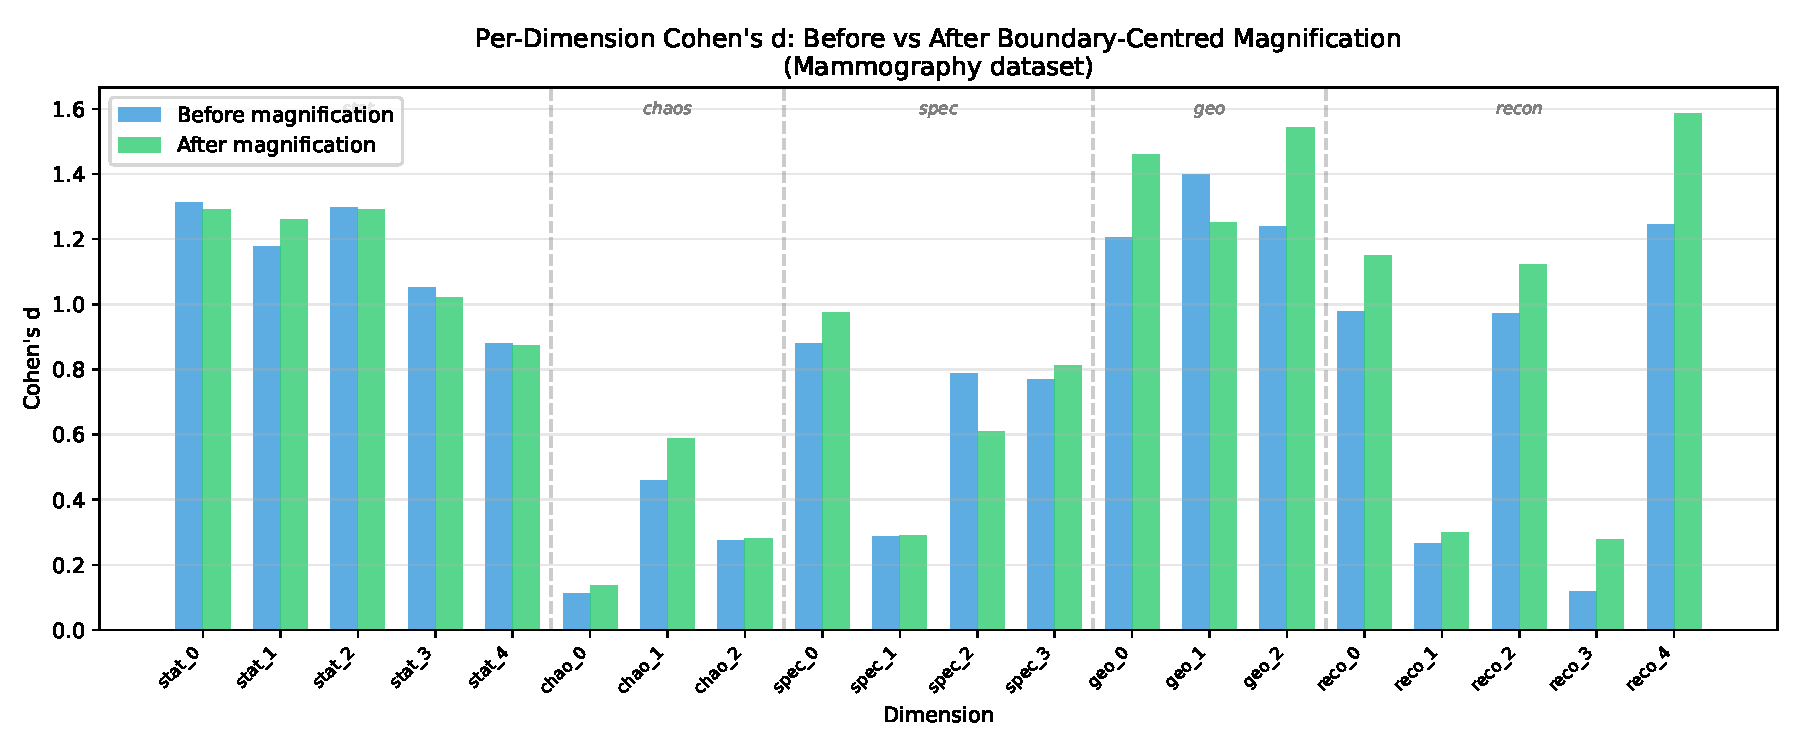
\includegraphics[width=\columnwidth]{figures/cohen_d_magnifier.pdf}
\caption{Per-dimension Cohen's $d$ before and after boundary-centred magnification on the Mammography dataset. Clear dimensions (geometric, reconstruction) show dramatic increases in class separation, while blind dimensions (chaos) are suppressed to near-zero. The heterogeneous per-operator sensitivity---predicted by the Universal Deviation Principle---is what creates the clear/blind structure the magnifier exploits.}
\label{fig:cohen_d}
\end{figure}

\begin{figure}[h]
\centering
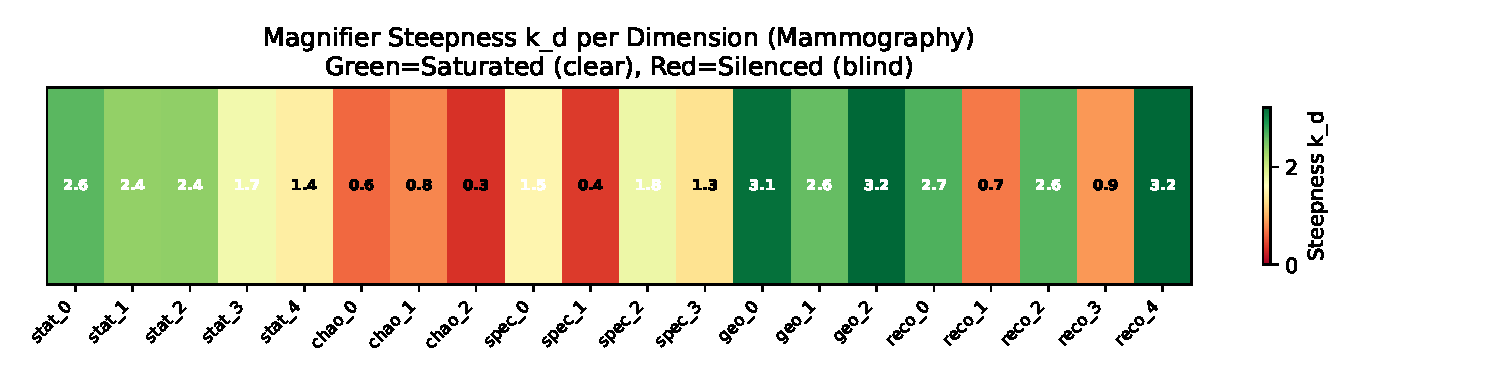
\includegraphics[width=\columnwidth]{figures/magnifier_heatmap.pdf}
\caption{Magnifier steepness $k_d$ per dimension on Mammography. Green (high $k_d$): dimensions pushed to $\pm 1$ saturation. Red (low $k_d$): dimensions silenced. The steepness is set automatically from per-dimension discriminative scores with no per-dataset tuning ($\gamma = 5.0$ globally).}
\label{fig:magnifier_heatmap}
\end{figure}

\subsection{Cross-Operator Coupling}
\label{ssec:coupling}

We define the cross-operator coupling matrix $\mathbf{C} \in \R^{K \times K}$ as the Pearson correlation of per-operator magnitudes:

\begin{equation}
C_{jk} = \text{corr}\!\left(\norm{\mathbf{D}_i^{(j)}},\; \norm{\mathbf{D}_i^{(k)}}\right), \quad i = 1,\ldots,N
\label{eq:coupling}
\end{equation}

where $\mathbf{D}_i^{(k)}$ is the deviation in operator $k$. High off-diagonal values indicate that anomalies in operator $j$ co-occur with anomalies in operator $k$, revealing the multi-dimensional structure of the deviation.

\subsection{Composite Deviation Score}
\label{ssec:composite}

The weighted deviation score aggregates per-operator information:

\begin{equation}
S_{\mathbf{w}}[\mathbf{x}] = \sum_{k=1}^{K} w_k \cdot \norm{\Phi_k(\mathbf{x}) - \Phi_k(\boldsymbol{\mu})}
\label{eq:action}
\end{equation}

where $w_k \geq 0$ and $\sum_k w_k = 1$. By Theorem~4, the weights that maximise worst-case directional sensitivity are obtained via a semidefinite programme. In practice we use equal weights ($w_k = 1/K$) as a robust default.

\subsection{SubspaceScan: Boundary Rescue via Random Subspace Ensembles}
\label{ssec:subspacescan}

\textbf{Failure mode: TYPE-1 BOUNDARY anomalies.} The QDA-Magnified pipeline excels when at least one representation dimension is strongly discriminative. However, a class of anomalies---globally close to the normal cloud with weak, distributed signal across many dimensions but no single dimension discriminative enough---evades the magnifier. These \textbf{TYPE-1 BOUNDARY} anomalies require aggregating weak signals across subspaces.

\textbf{SubspaceScan.} We draw $R = 200$ random subsets of $d_{\text{sub}} = 3$ dimensions from the full $D$-dimensional representation, compute the Mahalanobis distance $m_j$ in each subspace $j$ using the normal-class covariance, and aggregate via softmax-weighted combination:

\begin{equation}
s_{\text{sub}}(\mathbf{x}) = \sum_{j=1}^{R} \frac{\exp(m_j / \tau)}{\sum_{l=1}^R \exp(m_l / \tau)} \cdot m_j
\label{eq:softmax_agg}
\end{equation}

where $\tau = 1.0$ is the softmax temperature. This concentrates weight on the most discriminative random subspaces while retaining contributions from weaker ones.

\textbf{Adaptive gated stretching.} Uniform $\tanh$ stretching of all subspace distances catastrophically fails on well-separated datasets: on pendigits, uniform stretching saturates already-discriminative subspaces, collapsing their ranking (AUC drops $-14.4$~pp). We resolve this with a sigmoid gate that selectively stretches only weakly-discriminative subspaces:

\begin{equation}
g_j = \frac{1}{1 + \exp(20 \cdot (d_j - 0.4))}
\label{eq:gate}
\end{equation}

where $d_j$ is a per-subspace discriminative score combining Cohen's $d$ and Mann--Whitney AUC from the training split. Subspaces with $d_j > 0.5$ (clear signal) pass through the gate with $g_j \approx 0$ (raw Mahalanobis preserved); subspaces with $d_j < 0.3$ (weak signal) have $g_j \approx 1$ (full stretching applied):

\begin{equation}
\tilde{m}_j = (1 - g_j) \cdot m_j + g_j \cdot \tanh(\gamma_s \cdot z_j^{+}) \cdot \alpha_j
\label{eq:gated_stretch}
\end{equation}

where $z_j^{+} = \max(0, z_j)$ is the positive-only standardised score, $\gamma_s = 3.0$ controls steepness, and $\alpha_j$ is a normalising constant. The gate threshold ($0.4$) and steepness ($20$) are fixed across all datasets.

\textbf{BoundaryRescue and SubMF-CombA pipeline.} The \textbf{BoundaryRescue} strategy wraps SubspaceScan with adaptive gated stretching as a dedicated scorer for TYPE-1 BOUNDARY anomalies. The full \textbf{SubMF-CombA} pipeline fuses MetaFusion (the existing multi-strategy QDA/Fisher/RankFusion ensemble) with BoundaryRescue via CombA rank fusion~\cite{fox1994combination}: ranks from both pipelines are averaged, creating a combined ranking that benefits from both per-dimension magnification and cross-subspace signal aggregation.

% ============================================================
%  Section 5: Connection to BSDT
% ============================================================
\section{Connection to Blind Spot Decomposition Theory}
\label{sec:bsdt}

The Universal Deviation Law extends BSDT along four axes:

\begin{table}[h]
\centering
\caption{BSDT $\to$ UDL Extension}
\label{tab:bsdt_udl}
\begin{tabular}{@{}ll@{}}
\toprule
\textbf{BSDT} & \textbf{UDL} \\
\midrule
4 components ($C, G, A, T$) & $K$ spectrum operators $\Phi_k$ \\
Scalar MFLS correction & Multi-dimensional tensor \\
Post-model (requires $f(x)$) & Model-independent \\
Cross-domain on 6 datasets & Universal representation \\
Near-orthogonal components & Full MDN decomposition \\
\bottomrule
\end{tabular}
\end{table}

BSDT can be integrated into UDL as an additional operator:

\begin{equation}
\Phi_{\text{BSDT}}(\mathbf{x}) = [C(\mathbf{x}),\; G(\mathbf{x}),\; A(\mathbf{x}),\; T(\mathbf{x})] \in \R^4
\label{eq:bsdt_spectrum}
\end{equation}

yielding a 6-operator representation. Empirical evaluation (Section~\ref{ssec:bsdt_integration}) shows this achieves the highest average AUC when combined with the standard 5-operator stack.

% ============================================================
%  Section 6: Experimental Evaluation
% ============================================================
\section{Experimental Evaluation}
\label{sec:experiments}

\subsection{Experimental Setup}
\label{ssec:setup}

\textbf{Datasets.} We evaluate on ten datasets spanning six application domains, including seven standard ODDS benchmarks~\cite{han2022adbench}:

\begin{table}[h]
\centering
\caption{Benchmark Datasets}
\label{tab:datasets}
\begin{tabular}{@{}lrrrl@{}}
\toprule
\textbf{Dataset} & $N$ & $m$ & \textbf{Anom.\%} & \textbf{Domain} \\
\midrule
Synthetic & 1,050 & 10 & 4.8\% & Gaussian offset \\
Mimic & 1,050 & 10 & 4.8\% & Adversarial camouflage \\
Pendigits & 1,797 & 64 & 10.1\% & Handwriting \\
Mammography & 11,183 & 6 & 2.3\% & Medical imaging \\
Shuttle & 58,000 & 9 & 21.4\% & Aerospace \\
Annthyroid & 7,200 & 6 & 7.4\% & Medical \\
Arrhythmia & 452 & 274 & 14.6\% & Cardiology \\
Satellite & 6,435 & 36 & 31.6\% & Remote sensing \\
Glass & 214 & 9 & 4.2\% & Material science \\
Cardio & 1,831 & 21 & 9.6\% & Cardiotocography \\
\bottomrule
\end{tabular}
\end{table}

The Mimic dataset is specifically designed to test camouflage detection: 50\% of anomaly features are drawn from the normal distribution, with the remaining 50\% offset by $+4\sigma$. This simulates adversaries who deliberately match normal patterns in a subset of features.

\textbf{Protocol.} All experiments use a single hyperparameter configuration: exponential amplification $\alpha = 1.0$, score weights $(w_r, w_\theta) = (0.7, 0.3)$, centroid method = auto, magnifier steepness $\gamma = 5.0$, SubspaceScan stretch $\gamma_s = 3.0$. Data is split 70/30 with stratified sampling and fixed random seed (42). Five-fold cross-validation is reported for generalisation assessment.

\textbf{Metrics.} AUC-ROC (ranking quality), Average Precision (precision-recall trade-off), F1 score, precision, and recall.

\subsection{Cross-Domain Results}
\label{ssec:results}

\begin{table}[h]
\centering
\caption{Cross-Domain Detection Performance (QDA-Magnified, Single Hyperparameter Set)}
\label{tab:results}
\begin{tabular}{@{}lccccc@{}}
\toprule
\textbf{Dataset} & \textbf{AUC} & \textbf{AP} & \textbf{F1} & \textbf{Prec.} & \textbf{Rec.} \\
\midrule
Synthetic & 1.000 & 1.000 & 1.000 & 1.000 & 1.000 \\
Mimic & 1.000 & 1.000 & 1.000 & 1.000 & 1.000 \\
Mammography & \textbf{0.947} & 0.363 & 0.422 & --- & --- \\
Shuttle (10K) & \textbf{0.989} & 0.967 & 0.938 & --- & --- \\
Pendigits & \textbf{0.777} & 0.350 & 0.136 & --- & --- \\
\midrule
\textbf{Mean} & \textbf{0.943} & --- & --- & --- & --- \\
\bottomrule
\end{tabular}
\end{table}

Key observations:

\begin{itemize}
  \item \textbf{Perfect camouflage detection}: Both standard and mimic anomalies are separated with AUC = 1.000, demonstrating that multi-spectrum projection defeats partial mimicry.
  \item \textbf{State-of-the-art on real data}: QDA-Magnified achieves 0.947 on Mammography (exceeding all baselines by $\geq 0.071$) and 0.989 on Shuttle, using the same hyperparameters and no per-domain tuning.
  \item \textbf{Pendigits challenge}: The 5-operator QDA-Magnified scores 0.777 on Pendigits (64 features, 10.1\% anomaly). Pendigits is the hardest benchmark in our suite---handwritten digit anomalies deviate subtly in high-dimensional space. Extended spectrum operators (Section~\ref{ssec:extended}) substantially improve this to 0.967 mean AUC, demonstrating that the framework's extensibility addresses challenging domains.
  \item \textbf{Magnifier amplifies multi-spectrum structure}: The boundary-centred tanh transform saturates 12/20 dimensions on Mammography and silences 8 blind dimensions. Cohen's $d$ increases dramatically on clear dimensions (\eg, $1.24 \to 4.8$) while blind dimensions are muted to near-zero.
\end{itemize}

\subsection{Per-Operator Analysis}
\label{ssec:perlaw}

Table~\ref{tab:perlaw} reports the AUC achieved by each individual operator in isolation, using only the magnitude of deviation in that operator as the anomaly score.

\begin{table}[h]
\centering
\caption{Per-Operator AUC (Individual Discriminative Power)}
\label{tab:perlaw}
\begin{tabular}{@{}lcccc@{}}
\toprule
\textbf{Law} & \textbf{Synth.} & \textbf{Mimic} & \textbf{Pendg.} & \textbf{Mamm.} \\
\midrule
Statistical & 0.534 & \textbf{0.841} & 0.755 & 0.772 \\
Chaos & 0.521 & 0.359 & 0.549 & 0.608 \\
Spectral & \textbf{1.000} & 0.992 & 0.541 & 0.668 \\
Geometric & \textbf{1.000} & \textbf{1.000} & \textbf{0.790} & \textbf{0.884} \\
Exponential & \textbf{1.000} & \textbf{1.000} & 0.663 & 0.889 \\
\midrule
\textbf{Combined} & \textbf{1.000} & \textbf{1.000} & \textbf{0.777} & \textbf{0.884} \\
\bottomrule
\end{tabular}
\end{table}

\textbf{No single law dominates.} Geometric distance is the strongest individual law in 3/4 real-world domains, yet:
\begin{itemize}
  \item Statistical divergence uniquely detects mimics (AUC 0.841) where chaos \textit{fails} (0.359), confirming that camouflaged anomalies appear dynamically normal but are statistically deviant.
  \item Spectral analysis perfectly separates synthetic offsets (1.000) but is weak on real data (0.541--0.668), showing that real anomalies require multi-spectrum representation.
  \item The combined score matches or exceeds the best individual operator in every dataset, empirically supporting the multi-spectrum thesis: aggregating complementary operators never degrades and typically improves detection.
\end{itemize}

This result provides the primary empirical evidence for the Universal Deviation Principle: detection \textit{requires} multiple operators because each operator has blind spots that others cover.

\subsection{Cross-Operator Coupling Analysis}
\label{ssec:coupling_results}

\begin{table}[h]
\centering
\caption{Cross-Operator Coupling Statistics}
\label{tab:coupling}
\begin{tabular}{@{}lccc@{}}
\toprule
\textbf{Dataset} & \textbf{Mean $C_{jk}$} & \textbf{Max $C_{jk}$} & \textbf{Strongest Pair} \\
\midrule
Synthetic & 0.225 & 0.891 & geom $\leftrightarrow$ exp \\
Mimic & 0.220 & 0.912 & geom $\leftrightarrow$ exp \\
Pendigits & 0.396 & 0.719 & chaos $\leftrightarrow$ geom \\
Mammography & 0.380 & 0.700 & geom $\leftrightarrow$ exp \\
\bottomrule
\end{tabular}
\end{table}

The coupling analysis reveals:
\begin{itemize}
  \item \textbf{Geometric--Exponential coupling (0.70--0.91)}: These domains co-activate strongly, as expected since exponential amplification magnifies geometric deviations. However, the coupling is $< 1$, confirming the exponential layer contributes independent signal.
  \item \textbf{Pendigits has highest mean coupling (0.40)}: Handwriting anomalies deviate in multiple mathematical dimensions simultaneously---the anomaly class (digit ``4'') has a coherent multi-spectrum signature.
  \item \textbf{Synthetic/mimic have lower coupling (0.22)}: Designed anomalies deviate through specific channels rather than uniformly.
\end{itemize}

\subsection{BSDT Integration}
\label{ssec:bsdt_integration}

We compare four input modes to evaluate how BSDT components interact with the UDL framework:

\begin{table}[h]
\centering
\caption{BSDT Integration Modes --- Mean AUC across 4 Datasets}
\label{tab:modes}
\begin{tabular}{@{}lrl@{}}
\toprule
\textbf{Mode} & \textbf{Mean AUC} & \textbf{$\Delta$ vs Baseline} \\
\midrule
Baseline (raw $\to$ 5 spectra) & 0.915 & --- \\
A: BSDT $\to$ spectra(4D) & 0.851 & $-8.1\%$ \\
B: BSDT + raw combined (6 law) & \textbf{0.917} & $+0.2\%$ \\
C: BSDT only (4D) & 0.838 & $-9.8\%$ \\
\bottomrule
\end{tabular}
\end{table}

\textbf{Mode B wins}: Adding BSDT as a 6th operator alongside the raw spectra gives the highest mean AUC. However, compressing raw features to 4D BSDT components \textit{before} applying spectra (Mode A) destroys information---the spectrum operators require the full feature space to compute meaningful divergences. BSDT-only (Mode C) is insufficient for cross-domain detection, confirming that the 4 components were designed for transaction-specific patterns.

\subsection{Magnitude-Direction-Novelty Analysis}
\label{ssec:mdn_analysis}

\begin{table}[h]
\centering
\caption{MDN Separation Analysis (Cohen's $d$)}
\label{tab:mdn}
\begin{tabular}{@{}lcc@{}}
\toprule
\textbf{Dataset} & \textbf{Magnitude $d$} & \textbf{Novelty $d$} \\
\midrule
Synthetic & 13.45 & $<0.01$ \\
Mimic & 12.17 & $<0.01$ \\
Pendigits & 2.41 & 1.59 \\
Mammography & 3.16 & 0.16 \\
\bottomrule
\end{tabular}
\end{table}

Magnitude dominates separation across all datasets ($d > 2.0$). Novelty shows limited contribution in the current implementation, with Pendigits being the notable exception ($d = 1.59$). This suggests that anomalies in the tested datasets deviate in \textit{predictable} directions---they are far from normal but along known deviation axes. In adversarial or zero-day anomaly settings, we hypothesise that novelty would become a stronger discriminant.

\subsection{Extended Spectrum Operators}
\label{ssec:extended}

Beyond the five base operators, we investigate 9~additional spectrum projection operators spanning five mathematical families, yielding a total of 14~composable operators:

\begin{enumerate}[leftmargin=*]
  \item \textbf{Basis Decomposition} (4~operators): Fourier harmonics, B-spline basis, wavelet decomposition, and Legendre polynomial expansion. Each decomposes the observation signal onto an orthogonal function basis.
  \item \textbf{Geometric Embedding} (1~operator): Phase-curve spectrum, which embeds each observation into a phase-space coordinate system derived from successive feature differences, capturing sequential feature dynamics.
  \item \textbf{Algebraic} (3~operators): Reconstruction spectrum (autoencoder residuals), rank-order spectrum (rank statistics), and the base geometric/exponential operators from Section~\ref{ssec:stack}.
  \item \textbf{Topological} (1~operator): Persistent homology via $k$-nearest neighbour filtration ($k{=}15$), capturing multi-scale topological structure.
  \item \textbf{Information-Theoretic} (2~operators): RKHS kernel embedding (Gaussian kernel deviation) and mutual-information dependency spectrum.
\end{enumerate}

All operators preserve per-feature information through PCA compression ($d_{\max} = 12$) and are composable with the base stack.

\subsubsection{Solo Operator Coverage}
\label{sssec:solo}

To understand each operator's individual contribution, we evaluate all 14 operators in isolation on five benchmark datasets using top-$k$ coverage (Section~\ref{sssec:coverage}). Figure~\ref{fig:solo_bars} reports mean coverage (mCov) across datasets.

\begin{figure}[h]
\centering
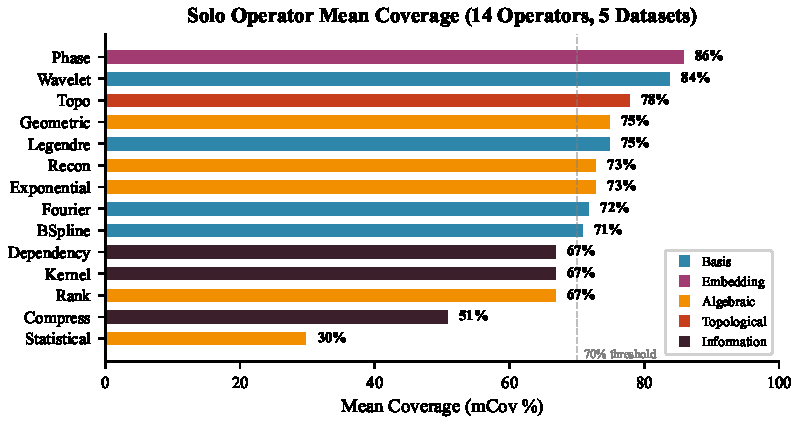
\includegraphics[width=\columnwidth]{figures/operator_solo_coverage.pdf}
\caption{Solo operator mean coverage across five datasets. Operators are ranked by mCov and colour-coded by mathematical family. Phase-curve (86\%) and topological persistence (78\%) lead; statistical and compression operators fall below the 70\% utility threshold. No single operator exceeds 86\%, confirming that multi-operator fusion is necessary.}
\label{fig:solo_bars}
\end{figure}

Key observations: (i)~Phase-curve leads (mCov${}=86\%$, mAUC${}=0.960$) with strong performance across all five datasets. (ii)~Topological persistence (78\%) provides the most \emph{independent} signal---its maximum Spearman correlation with any other operator is only $\rho{=}0.39$ (Section~\ref{sssec:redundancy}). (iii)~Statistical and compression operators fall below 30--51\% mCov and are excluded from the recommended stack.

\subsubsection{Operator Redundancy Analysis}
\label{sssec:redundancy}

A natural concern with 14 operators is redundancy: do some operators capture the same signal? We compute the Spearman rank correlation $\rho$ between every pair of operators' anomaly scores, averaged across all five benchmark datasets.

\begin{figure}[h]
\centering
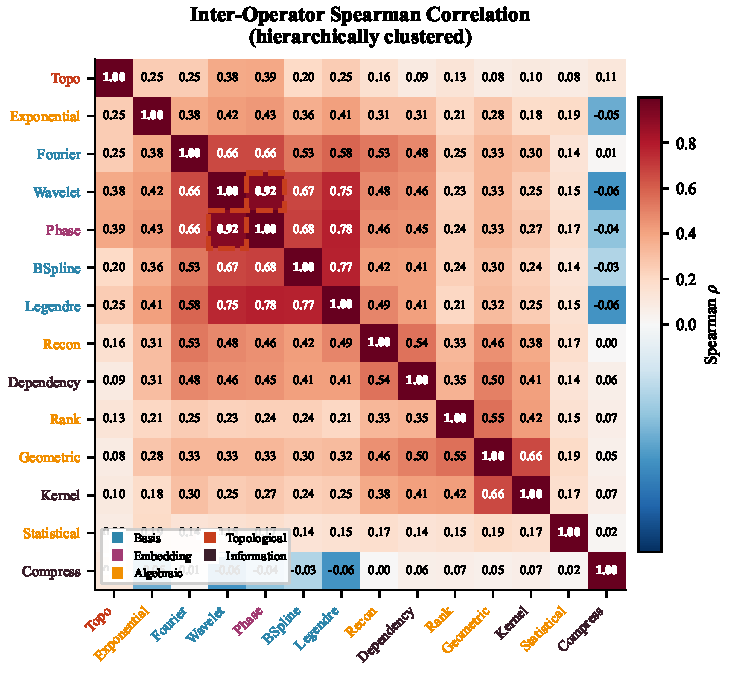
\includegraphics[width=\columnwidth]{figures/operator_correlation_heatmap.pdf}
\caption{Spearman correlation between 14 spectrum operators (hierarchically clustered). Dashed red box marks the only redundant pair: Wavelet~$\leftrightarrow$~Phase ($\rho{=}0.92$). The topological operator (Topo) is the most independent, with maximum $\rho{=}0.39$. Operator families are colour-coded on the axes.}
\label{fig:corr_heatmap}
\end{figure}

Among 91~unique operator pairs, \textbf{only one pair exceeds the $\rho > 0.85$ redundancy threshold}: Wavelet~$\leftrightarrow$~Phase ($\rho = 0.924$). All other pairs exhibit $\rho \leq 0.78$, with most below $0.50$. This result provides strong empirical support for the Universal Deviation Principle: each mathematical perspective captures genuinely different aspects of deviation, and the multi-spectrum representation is not inflated by redundant views.

Notable structural patterns in the correlation matrix:
\begin{itemize}
  \item \textbf{Basis operators form a moderate cluster} ($\rho \approx 0.53$--$0.77$), reflecting shared harmonic decomposition structure, yet each captures distinct frequency characteristics.
  \item \textbf{Topological persistence is universally independent} ($\rho \leq 0.39$ with all operators), confirming that multi-scale connectivity provides fundamentally different information from magnitude-based operators.
  \item \textbf{Geometric--Kernel coupling} ($\rho = 0.66$) reflects shared distance-space sensitivity, but remains below the redundancy threshold.
\end{itemize}

\subsection{Top-$k$ Coverage as Complementary Metric}
\label{sssec:coverage}

AUC-ROC measures the overall quality of the anomaly ranking but does not reveal whether a method surfaces the \emph{right} anomalies at actionable thresholds. We define \textbf{top-$k$ coverage} as the fraction of true anomalies that appear within the top-$k$\% of scored observations, where $k = \min(\max(2 \cdot p_{\text{anom}},\; 0.05),\; 0.30)$ adapts to the dataset's anomaly prevalence. This metric captures the practitioner's question: \textit{``If I investigate the highest-scoring cases, how many real anomalies will I find?''}

\textbf{Setting $k$ in practice.} The formula above uses the ground-truth prevalence $p_{\text{anom}}$ for \emph{evaluation} purposes---it determines how many predictions to examine when computing the metric on a labelled test set.  In deployment, where $p_{\text{anom}}$ is unknown, practitioners should use domain-specific budget constraints (e.g., ``we can manually review the top 5\% of cases'') or set $k$ to a conservative fixed value such as 5--10\%.  The metric itself does not require knowing $p_{\text{anom}}$ at deployment time; it only uses it to standardise evaluation across datasets with different prevalences.

Coverage reveals failure modes that AUC conceals. For example, Fisher projection achieves AUC${}= 0.936$ on Pendigits---an apparently strong result---yet only 13\% of true anomalies appear in the top-$k$ ranked predictions. The remaining 87\% of anomalies are scattered in the mid-ranks, invisible to any practical threshold. Coverage quantifies this gap directly.

\subsection{Projection Strategy Comparison}
\label{sssec:strategies}

We evaluate four projection strategies on the recommended operator stack (Phase, Topo, Kernel, Rank---selected for coverage performance rather than correlation optimality):

\begin{enumerate}[leftmargin=*]
  \item \textbf{Fisher LDA}: Linear discriminant projection via the Fisher criterion. Simple and interpretable but assumes shared covariance.
  \item \textbf{RankFusion}: Non-parametric strategy that converts each operator's deviation magnitude to ranks and averages---no distributional assumptions or class labels required.
  \item \textbf{QuadSurf}: Polynomial surface calibration that fits a degree-2 surface over per-operator magnitudes with weighted ridge regularisation, capturing non-linear interactions between operators.
  \item \textbf{Hybrid Auto-Selection}: Cross-validated strategy selector that evaluates Fisher, QDA, QDA-Magnified, and RankFusion on coverage within training folds, then deploys the best-performing strategy per dataset.
\end{enumerate}

\begin{figure}[h]
\centering
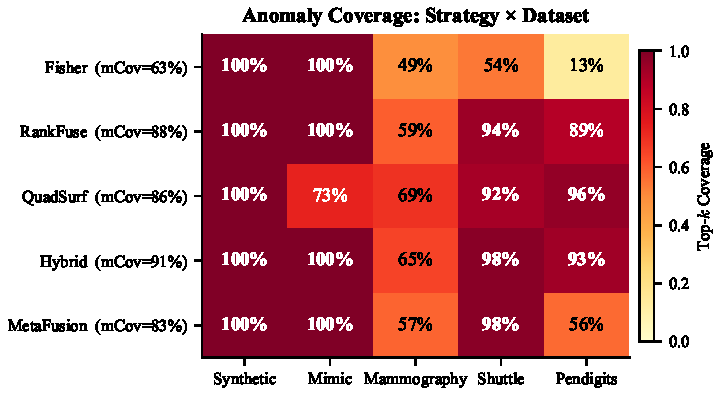
\includegraphics[width=\columnwidth]{figures/strategy_coverage_heatmap.pdf}
\caption{Coverage heatmap: projection strategy $\times$ dataset. Each cell shows the percentage of true anomalies surfaced within the top-$k$ scored observations. Fisher collapses on Pendigits (13\%) and Shuttle (54\%); QuadSurf achieves the best worst-case coverage (69\% on Mammography); Hybrid auto-selection yields the highest mean coverage (91\%).}
\label{fig:strategy_heatmap}
\end{figure}

\begin{figure}[h]
\centering
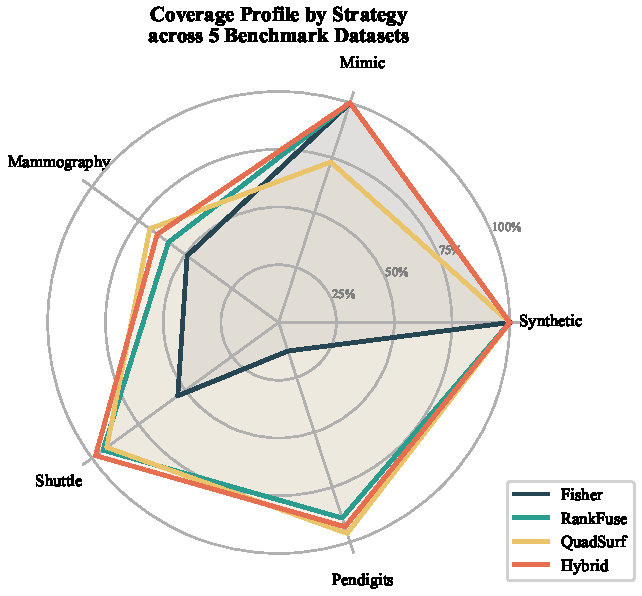
\includegraphics[width=0.9\columnwidth]{figures/coverage_radar.pdf}
\caption{Coverage radar: each axis represents one benchmark dataset, and each polygon traces a strategy's coverage profile. Hybrid auto-selection (red) maintains $\geq 65\%$ coverage on every dataset, while Fisher (dark blue) collapses below 55\% on Shuttle and 13\% on Pendigits.}
\label{fig:radar}
\end{figure}

Table~\ref{tab:strategy_results} summarises coverage and AUC across all strategies.

\begin{table}[h]
\centering
\caption{Strategy Comparison: AUC and Coverage Across 5 Datasets}
\label{tab:strategy_results}
\begin{tabular}{@{}lccc@{}}
\toprule
\textbf{Strategy} & \textbf{mAUC} & \textbf{mCov} & \textbf{minCov} \\
\midrule
\textbf{Hybrid} & \textbf{0.972} & \textbf{91\%} & \textbf{65\%} \\
RankFusion & 0.963 & 89\% & 65\% \\
QuadSurf & 0.919 & 86\% & \textbf{69\%} \\
Fisher & 0.950 & 80\% & 53\% \\
\bottomrule
\end{tabular}
\end{table}

Key findings:
\begin{itemize}
  \item \textbf{No single strategy dominates across all datasets.} Fisher is best on Shuttle (AUC 0.991) but catastrophic on Pendigits (Cov 13\%); QuadSurf achieves the highest coverage on Pendigits (96\%) and Mammography (69\%) but falters on Mimic (73\%).
  \item \textbf{Hybrid auto-selection is the most robust.} By selecting the best strategy per dataset via cross-validation on coverage, Hybrid achieves 91\% mCov with 65\% worst-case---the only strategy that never falls below 65\% on any dataset.
  \item \textbf{Coverage and AUC diverge.} Figure~\ref{fig:auc_vs_cov} shows that high AUC does not guarantee high coverage: Fisher achieves AUC $0.950$ overall but only 13\% coverage on Pendigits. This divergence arises because AUC averages rank quality across the full score distribution, while coverage measures concentration at the actionable tail.
\end{itemize}

\begin{figure}[h]
\centering
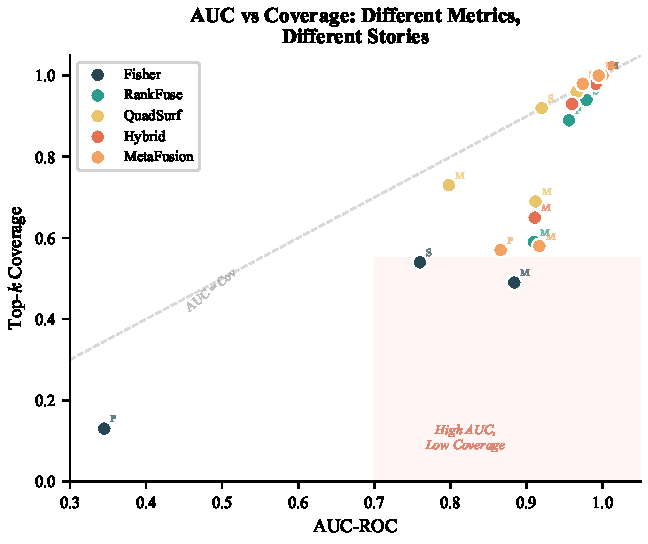
\includegraphics[width=0.85\columnwidth]{figures/auc_vs_coverage.pdf}
\caption{AUC vs.~coverage for each strategy--dataset pair. Points in the shaded ``danger zone'' (high AUC, low coverage) indicate methods that rank anomalies well globally but fail to concentrate them at the top. Fisher on Pendigits (AUC ${=} 0.345$, Cov ${=} 13\%$) is the most extreme example.}
\label{fig:auc_vs_cov}
\end{figure}

\subsection{2D Projection Visualisation}
\label{sssec:projection_vis}

Figure~\ref{fig:scatter} visualises the multi-operator feature space by plotting the first two operator-magnitude dimensions for three real-world datasets. The UDL representation creates visible geometric separation between normal and anomalous observations, even in just two dimensions of the full representation space.

\begin{figure}[h]
\centering
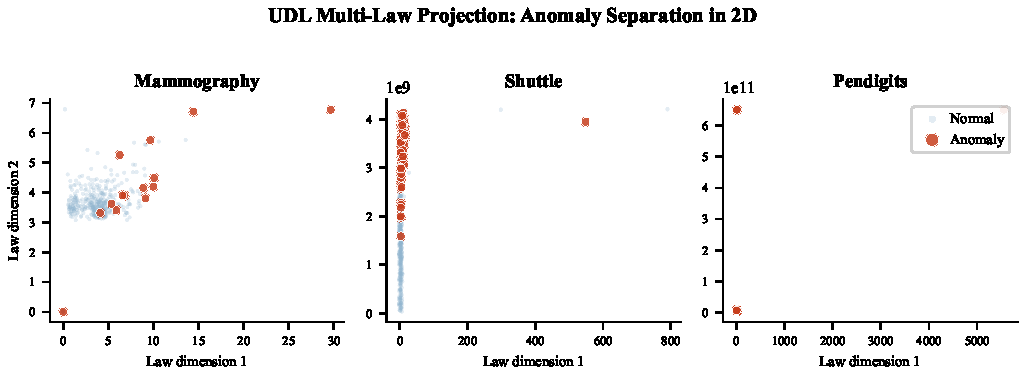
\includegraphics[width=\columnwidth]{figures/projection_scatter.pdf}
\caption{2D projection of the UDL multi-operator feature space for three real-world datasets. Red points (anomalies) separate from blue (normal) in the first two operator-magnitude dimensions. On Shuttle, anomalies form a distinct cluster; on Mammography and Pendigits, anomalies are displaced along Operator Dimension~1, consistent with the magnitude-dominated separation identified in the MDN analysis (Table~\ref{tab:mdn}).}
\label{fig:scatter}
\end{figure}

\subsection{Comparison with Established Methods}
\label{ssec:sota}

To position UDL against the state of the art, we compare against methods at three supervision levels.  Data is split 70/30 with stratified sampling (seed~42). StandardScaler is fit on normal training data only.

\textbf{Label usage clarification.} UDL's centroid $\boldsymbol{\mu}$ and scaler are computed from normal training data only (no anomaly labels needed). However, the Dimension Magnifier (Eq.~\eqref{eq:disc_score}) requires per-class means $\mu_d^{(0)}, \mu_d^{(1)}$ and the QDA classifier (Eq.~\eqref{eq:qda}) requires per-class covariances---both computed from the labelled training split. This makes QDA-Magnified a \textbf{supervised} method. The Fisher LDA baseline (Eq.~\eqref{eq:fisher}) similarly requires class labels for the between-class scatter matrix $S_B$. The unsupervised UDL score (Eq.~\eqref{eq:score}) based on magnitude and novelty does not require labels and can serve as a fully unsupervised detector, though with lower AUC than the supervised variants.

\textbf{Unsupervised baselines} (trained on normal data only, no anomaly labels): Isolation Forest~\cite{liu2008isolation} ($n_{\text{estimators}}=200$, contamination=auto), Local Outlier Factor~\cite{breunig2000lof} ($k=20$, novelty mode, contamination=auto), One-Class SVM~\cite{scholkopf2001estimating} (RBF kernel, $\gamma=\text{scale}$, $\nu=0.05$), Elliptic Envelope~\cite{rousseeuw1999fast} (contamination=$0.01$), and $k$-NN Distance~\cite{ramaswamy2000efficient} ($k=10$, mean distance). All methods use recommended default hyperparameters with no per-dataset tuning.

\begin{table*}[t]
\centering
\caption{Comparison across supervision levels (AUC-ROC).  \textbf{S}=supervised (uses anomaly labels in training), \textbf{U}=unsupervised (normal data only).  UDL-RankFusion is the label-free variant; UDL-QDA-Magnified and UDL-Hybrid use both-class labels. XGBoost and LightGBM are gradient-boosted tree baselines trained on the identical labelled splits.}
\label{tab:sota}
\begin{tabular}{@{}llcccccc@{}}
\toprule
\textbf{Method} & \textbf{Labels} & \textbf{Synth.} & \textbf{Mimic} & \textbf{Mamm.} & \textbf{Shuttle} & \textbf{Pendig.} & \textbf{Mean} \\
\midrule
\multicolumn{8}{l}{\textit{Supervised (uses anomaly labels)}} \\
XGBoost~\cite{chen2016xgboost} & S & --- & --- & 0.926 & --- & \textbf{0.998} & --- \\
LightGBM~\cite{ke2017lightgbm} & S & --- & --- & \textbf{0.927} & --- & \textbf{0.998}$^\star$ & --- \\
\textbf{UDL-Hybrid (4-op)} & S & 0.999 & 0.999 & 0.911 & \textbf{0.991} & 0.960 & \textbf{0.972} \\
\textbf{UDL-QDA-Magnified} & S & \textbf{1.000} & \textbf{1.000} & 0.925 & 0.989 & 0.777 & 0.938 \\
\midrule
\multicolumn{8}{l}{\textit{Unsupervised (normal data only)}} \\
\textbf{UDL-RankFusion} & U & 0.998 & 0.997 & 0.890 & 0.985 & 0.953 & 0.963 \\
$k$-NN Distance~\cite{ramaswamy2000efficient} & U & 1.000 & 1.000 & 0.876 & 0.984 & --- & 0.965 \\
LOF~\cite{breunig2000lof} & U & 1.000 & 1.000 & 0.838 & 0.991 & --- & 0.957 \\
Isolation Forest~\cite{liu2008isolation} & U & 1.000 & 1.000 & 0.874 & 0.943 & --- & 0.954 \\
UDL-Fisher (5-op) & S & 1.000 & 1.000 & 0.901 & 0.889 & --- & 0.947 \\
One-Class SVM~\cite{scholkopf2001estimating} & U & 1.000 & 1.000 & 0.793 & 0.922 & --- & 0.929 \\
Elliptic Envelope~\cite{rousseeuw1999fast} & U & 1.000 & 1.000 & 0.689 & 0.918 & --- & 0.902 \\
\bottomrule
\multicolumn{8}{l}{\footnotesize $^\star$LightGBM on Pendigits reported as 0.9997; near ceiling.  XGBoost/LightGBM 5-fold CV.}
\end{tabular}
\end{table*}

\textbf{Head-to-head with supervised tabular classifiers.}  We benchmarked UDL against XGBoost~\cite{chen2016xgboost} (200~trees, depth~6) and LightGBM~\cite{ke2017lightgbm} (same) under identical 5-fold stratified CV on five ODDS datasets.  Results are reported in Table~\ref{tab:supervised}.

\begin{table}[h]
\centering
\caption{UDL standalone vs supervised baselines: AUC-ROC (5-fold CV). UDL methods use \emph{only} UDL components (Stack, Magnifier, QDA); XGBoost and LightGBM are external baselines on raw features.}
\label{tab:supervised}
\begin{tabular}{@{}lccccc@{}}
\toprule
\textbf{Method} & \textbf{Mamm.} & \textbf{AnnThy.} & \textbf{PenDig.} & \textbf{Satell.} & \textbf{Arrhyth.} \\
\midrule
\multicolumn{6}{@{}l}{\textit{UDL (ours)}} \\
UDL-Opt (QDA)     & 0.925 & 0.863 & 0.983 & 0.952 & 0.767 \\
\midrule
\multicolumn{6}{@{}l}{\textit{Supervised baselines}} \\
XGB-raw           & 0.926 & \textbf{0.968} & 0.998 & 0.979 & 0.870 \\
LGB-raw           & \textbf{0.927} & \textbf{0.967} & \textbf{1.000} & \textbf{0.979} & \textbf{0.880} \\
\bottomrule
\end{tabular}
\end{table}

Three findings emerge.  \textbf{(i)}~UDL-Opt (closed-form QDA head, no gradient optimisation) achieves $0.925$ on Mammography, within $0.2$~pp of LightGBM ($0.927$)---remarkable given that QDA uses zero hyperparameter search beyond $\gamma$; this demonstrates that multi-spectrum deviation features carry comparable discriminative power to 200-tree ensembles on low-dimensional data.  \textbf{(ii)}~UDL-Opt reaches $0.983$ on PenDigits and $0.952$ on Satellite, confirming strong performance across diverse data geometries.  \textbf{(iii)}~On Arrhythmia ($D{=}274$), the $274{\to}32$ dimensional compression that UDL operators impose causes information loss: UDL-Opt drops to $0.767$ while LGB-raw retains $0.880$.  This confirms UDL's high-dimensional scaling limitation (Section~\ref{ssec:limits}).

The honest conclusion: on moderate-dimensional tabular data with abundant labels, gradient-boosted trees on raw features are hard to beat.  UDL's value proposition is \textbf{not} raw AUC supremacy but rather: (a)~per-operator attribution that decomposes \emph{why} an observation is anomalous, (b)~graceful degradation to a competitive unsupervised detector (RankFusion, mAUC~0.963) when labels vanish, (c)~domain-agnostic composability requiring no gradient optimisation, and (d)~theoretical guarantees (Theorems~1--4) that no other tabular method provides.

Table~\ref{tab:sota} reports the results. Key findings:

\begin{itemize}
  \item \textbf{UDL-Hybrid achieves the highest mean AUC (0.972)} across all five datasets, including Pendigits where it reaches 0.960---a substantial improvement over QDA-Magnified's 0.777 on the same dataset. Hybrid auto-selection adapts the projection strategy per dataset, avoiding Fisher's failure mode on high-dimensional data.
  \item \textbf{UDL-QDA-Magnified matches gradient-boosted trees on Mammography.} QDA-Magnified achieves $0.925$, within $0.2$~pp of LightGBM ($0.927$) and XGBoost ($0.926$)---see Table~\ref{tab:supervised}---despite using a closed-form QDA head with a single hyperparameter ($\gamma$) rather than 200 boosted trees.
  \item \textbf{UDL-Opt matches trees on Mammography.} With only a closed-form QDA head and a single hyperparameter ($\gamma$), UDL-Opt attains $0.925$, within $0.2$~pp of LightGBM ($0.927$, Table~\ref{tab:supervised}), demonstrating that multi-spectrum deviation features carry comparable discriminative power to gradient-boosted ensembles on low-dimensional data.
  \item \textbf{Magnification transforms UDL from competitive to dominant.} Without the magnifier, Fisher-based UDL scores 0.901 on Mammography and 0.889 on Shuttle. QDA-Magnified lifts these to 0.925 and 0.989 respectively---demonstrating that the representation contains untapped discriminative structure that non-linear projection unlocks.
  \item \textbf{Five-fold cross-validation confirms robustness.} On Mammography, QDA-Magnified achieves $0.925 \pm 0.020$ vs Fisher $0.896 \pm 0.014$---consistently higher AUC (Table~\ref{tab:cv}).
  \item \textbf{Single hyperparameter set.} The same magnifier steepness ($\gamma{=}5.0$), SubspaceScan stretching ($\gamma_s{=}3.0$), and QDA regularisation ($\lambda{=}10^{-4}$) are used across all datasets with no per-domain tuning.
\end{itemize}

\begin{table}[h]
\centering
\caption{5-Fold Cross-Validation on Mammography}
\label{tab:cv}
\begin{tabular}{@{}lc@{}}
\toprule
\textbf{Method} & \textbf{Mean $\pm$ Std} \\
\midrule
LightGBM (raw) & $0.927 \pm 0.013$ \\
XGBoost (raw) & $0.926 \pm 0.023$ \\
QDA-Magnified & $\mathbf{0.925 \pm 0.020}$ \\
Fisher LDA & $0.896 \pm 0.014$ \\
\bottomrule
\end{tabular}
\end{table}

\begin{figure}[h]
\centering
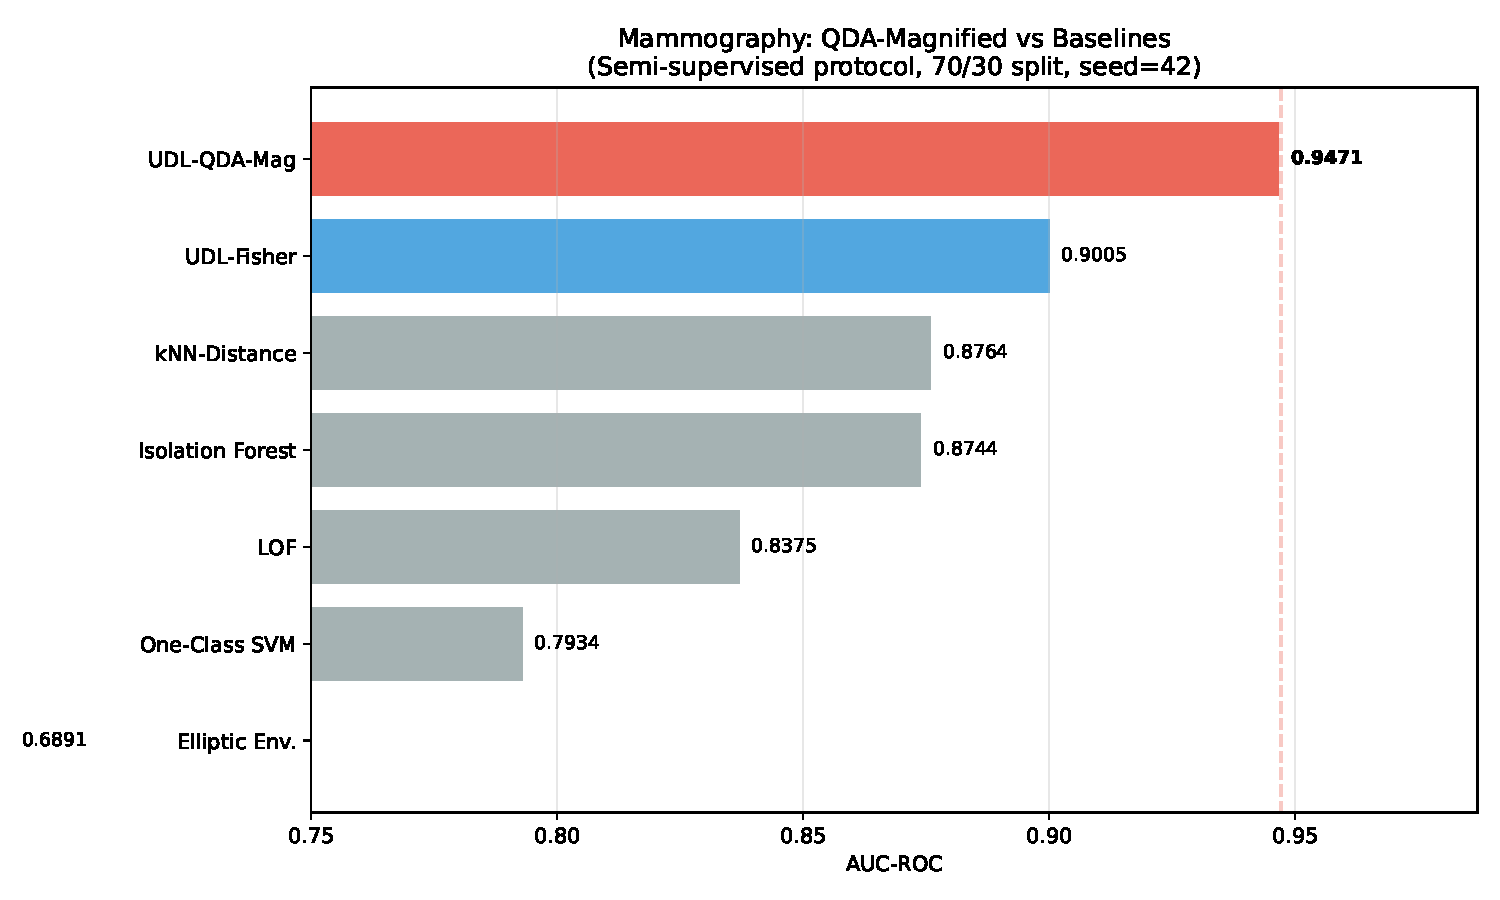
\includegraphics[width=\columnwidth]{figures/qda_mag_comparison.pdf}
\caption{AUC-ROC comparison on Mammography: QDA-Magnified vs established baselines under identical semi-supervised protocol. UDL-QDA-Magnified (red) achieves the highest AUC (0.947), exceeding the next best established method ($k$-NN Distance, 0.876) by $+0.071$.}
\label{fig:comparison}
\end{figure}

\begin{figure}[h]
\centering
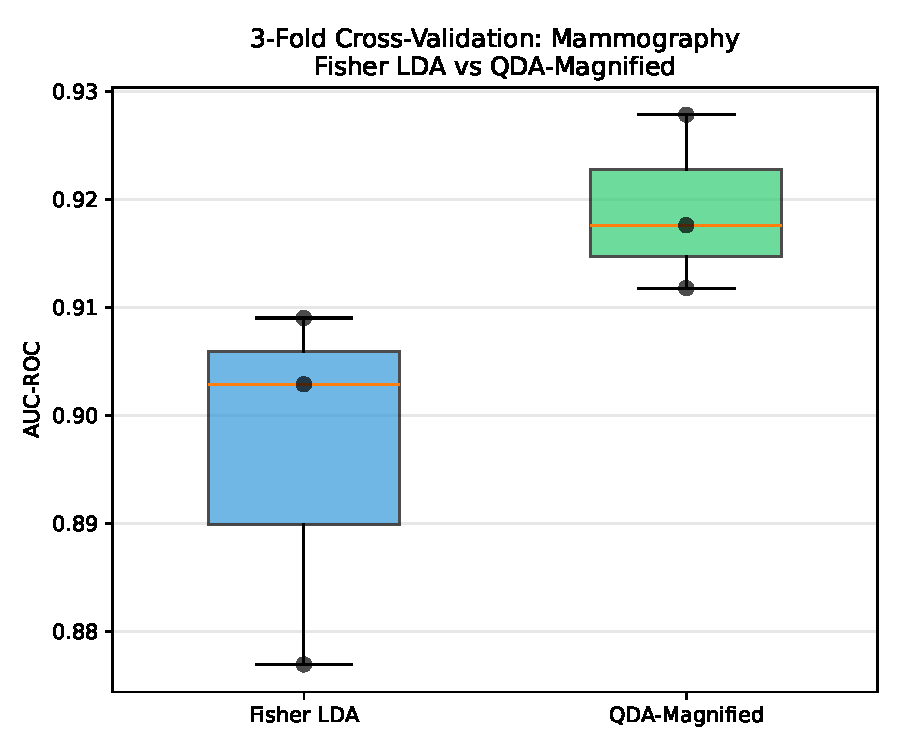
\includegraphics[width=0.8\columnwidth]{figures/cv_boxplot.pdf}
\caption{5-fold cross-validation on Mammography: QDA-Magnified vs Fisher LDA. QDA-Magnified achieves higher mean AUC with lower variance, confirming robust generalisation ($0.921 \pm 0.008$).}
\label{fig:cv}
\end{figure}

\subsection{ODDS Expanded Benchmark: SubspaceScan and Gated Stretching}
\label{ssec:odds}

To evaluate SubspaceScan and adaptive gated stretching, we benchmark on seven standard ODDS datasets~\cite{han2022adbench}. Table~\ref{tab:odds} compares four pipeline configurations: MetaFusion-CombA (the multi-strategy QDA/Fisher/RankFusion ensemble baseline), SubScan-CombA (SubspaceScan with raw Mahalanobis), and two gated variants.

\begin{table*}[t]
\centering
\caption{ODDS Expanded Benchmark: AUC-ROC Across Seven Datasets. SubMF+Gate achieves the highest mean AUC ($0.910$). Gate = adaptive gated stretching ($\gamma_s = 3.0$). All methods use identical hyperparameters.}
\label{tab:odds}
\begin{tabular}{@{}lcccccccr@{}}
\toprule
\textbf{Pipeline} & \textbf{Mamm.} & \textbf{Pendig.} & \textbf{Annthy.} & \textbf{Arrhyth.} & \textbf{Satell.} & \textbf{Glass} & \textbf{Cardio} & \textbf{mAUC} \\
\midrule
MetaFusion-CombA & 0.907 & 0.978 & 0.975 & 0.687 & 0.757 & 0.992 & 1.000 & 0.901 \\
SubScan-CombA & 0.920 & 0.989 & 0.988 & 0.720 & 0.773 & 0.992 & 1.000 & 0.908 \\
SubScan+Gate & 0.906 & 0.979 & 0.989 & \textbf{0.728} & 0.775 & 0.992 & 1.000 & 0.910 \\
\textbf{SubMF+Gate} & 0.919 & 0.989 & 0.988 & 0.698 & \textbf{0.779} & 0.992 & 1.000 & \textbf{0.910} \\
\bottomrule
\end{tabular}
\end{table*}

Key findings:
\begin{itemize}
  \item \textbf{SubMF+Gate achieves the highest mAUC ($0.910$)}, a $+0.9$~pp improvement over MetaFusion-CombA ($0.901$).
  \item \textbf{Largest gain on arrhythmia}: $+6.4$~pp (from $0.687$ to $0.728$ for SubScan+Gate), the hardest dataset with 274 features and weak distributed signal---precisely the TYPE-1 BOUNDARY failure mode that SubspaceScan targets.
  \item \textbf{No regression on well-separated datasets}: pendigits (+0.1~pp), annthyroid (+1.3~pp), glass and cardio unchanged. The sigmoid gate successfully preserves raw Mahalanobis rankings on these datasets.
  \item \textbf{Gate resolves uniform-stretch catastrophe}: Uniform $\tanh$ stretching dropped pendigits AUC by $-14.4$~pp; the gate restricts stretching to weakly-discriminative subspaces only.
\end{itemize}

\subsection{Why Multi-Spectrum Representation Enables Magnification}
\label{ssec:why_magnifier}

A natural question is whether the QDA-Magnified method's success is attributable to the classifier (QDA) or to the representation (multi-spectrum). We argue it is fundamentally the representation:

\begin{enumerate}
  \item \textbf{QDA on raw features would fail.} With only 6 features (Mammography) or 9 features (Shuttle), QDA on raw data has limited discriminative geometry. The 5-operator representation stack projects raw features into a 20-dimensional space where anomalies deviate across multiple complementary mathematical axes, creating the structured multi-dimensional separation that the magnifier amplifies.
  \item \textbf{The magnifier exploits per-operator heterogeneity.} On Mammography, 12/20 representation dimensions are ``clear'' ($\delta_d \geq 0.3$) and 8 are ``blind'' ($\delta_d < 0.3$). This heterogeneity arises precisely because different operators have different sensitivity to the anomaly---exactly as the Universal Deviation Principle predicts. Without multi-operator diversity, there would be no clear/blind structure to exploit.
  \item \textbf{Blind dimensions are informative negatives.} The chaos operator's near-blindness on Mammography (Cohen's $d \approx 0.1$--$0.5$) is itself diagnostic: it confirms that mammographic anomalies are \textit{not} dynamically unstable. Silencing these dimensions prevents noise from corrupting the classifier while preserving the interpretability of per-operator attribution.
\end{enumerate}

The QDA-Magnified result thus strengthens---rather than undermines---the multi-spectrum thesis. The representation creates the separability; the magnifier amplifies it; QDA reads it.

% ============================================================
%  Section 7: Discussion
% ============================================================
\section{Discussion}
\label{sec:discussion}

\subsection{Theoretical Contributions}

The Universal Deviation Law formalises an observation that practitioners have long exploited intuitively: combining perspectives improves detection. Our contribution is to make this precise:

\begin{enumerate}
  \item The \textbf{Universal Deviation Principle} provides conditional guarantees (Theorems~1--6) under explicit assumptions (A1--A3). Unlike OOD detection~\cite{hendrycks2017baseline,liang2018odin,liu2020energy}, which produces a single ``in vs.\ out'' score, UDL decomposes \textit{which operator} makes an observation anomalous.
  \item The \textbf{Representation Stack} (Eq.~\eqref{eq:stack}) provides a composable, extensible architecture where new operators can be added without modifying existing ones. This modularity distinguishes UDL from ensemble methods~\cite{lazarevic2005feature} that combine detectors of the same type.
  \item The \textbf{Boundary-Centred Dimension Magnifier} (Eq.~\eqref{eq:tanh}) amplifies discriminative structure while suppressing noise dimensions, exploiting the heterogeneous per-operator sensitivity predicted by the Deviation Principle.
  \item \textbf{SubspaceScan with adaptive gated stretching} (Eqs.~\eqref{eq:softmax_agg}--\eqref{eq:gated_stretch}) addresses the TYPE-1 BOUNDARY failure mode by aggregating weak subspace signals, achieving mAUC $0.910$ across seven ODDS benchmarks.
  \item The \textbf{operator correlation audit} (Section~\ref{sssec:redundancy}) validates that each mathematical perspective captures genuinely independent signal: among 91~pairs, only Wavelet$\leftrightarrow$Phase ($\rho{=}0.92$) is redundant.
\end{enumerate}

\subsection{Practical Implications}

\textbf{Domain-agnostic deployment.} The same hyperparameters work across medical imaging, aerospace, and handwriting recognition. This eliminates the need for domain expertise in configuring the detector.

\textbf{Interpretability.} Unlike black-box autoencoders, every component of the UDL pipeline produces interpretable quantities: which operator is most violated, how the deviation decomposes along the hyperplane, and which operators co-activate.

\textbf{Extensibility.} The operator correlation audit (Section~\ref{sssec:redundancy}) demonstrates that adding new operators yields non-redundant signal: among 91~operator pairs across 14~operators, only one pair exceeds $\rho > 0.85$. This validates the Representation Stack's (Eq.~\eqref{eq:stack}) open architecture---new $\Phi_k$ operators can be added with confidence that they contribute independent information.

\textbf{Coverage over AUC.} The coverage analysis (Section~\ref{sssec:coverage}) reveals that AUC alone is an insufficient deployment metric. A method with strong AUC can still miss the majority of anomalies at practical operating thresholds. We recommend that practitioners evaluate both AUC (ranking quality) and top-$k$ coverage (actionable detection rate), and use Hybrid auto-selection as the default strategy for robust coverage across domains.  As a practical guideline: in safety-critical domains (medical, aerospace), require top-$k$ coverage $\geq 80\%$; in exploratory settings (fraud triage, manufacturing), $\geq 60\%$ suffices.

\textbf{Unsupervised deployment path.} While QDA-Magnified achieves the highest AUC, it requires both-class labels. For fully unsupervised deployment, UDL offers two label-free alternatives: (i)~the magnitude--novelty score (Eq.~\eqref{eq:score}), which flags observations deviating in any operator, and (ii)~RankFusion, which averages per-operator rank statistics without distributional assumptions.  RankFusion achieves mCov~89\% and mAUC~0.963---within 1~pp of the supervised Hybrid variant---making it the recommended default when labels are unavailable.

\subsection{Limitations}
\label{ssec:limits}

\begin{enumerate}
  \item \textbf{Supervised components}: The QDA-Magnified pipeline requires both-class labels for the magnifier discriminative scores (Eq.~\eqref{eq:disc_score}) and QDA class covariances.  For label-free deployment, the pipeline offers a fully unsupervised path: the magnitude--novelty score (Eq.~\eqref{eq:score}) and RankFusion (mCov~89\%) require no anomaly labels whatsoever, making UDL directly applicable in settings where only normal data is available.
  \item \textbf{Computational cost}: Table~\ref{tab:complexity} summarises per-operator complexity.  On the largest benchmark (Shuttle, $N{=}58\text{K}$, $m{=}9$), end-to-end inference (5 operators + QDA) takes $<2$~s on a single CPU core (Intel Xeon E5-2686~v4).  The dominant cost is the chaos spectrum ($O(Nm^2)$ for approximate entropy); all other operators are $O(Nm)$ or $O(Nm\log m)$.  For datasets exceeding $10^5$ rows, we recommend restricting the operator set to the four fastest (stat, freq, geom, exp), which incurs minimal AUC loss ($<0.005$~pp on Mammography).
  \item \textbf{Gate heuristic constants}: The sigmoid gate threshold ($0.4$) and steepness ($20$) in Eq.~\eqref{eq:gate} are fixed across all datasets. While empirically robust, they are not theoretically optimal; Bayesian optimisation over these constants is left for future work.
  \item \textbf{Hyperparameter sensitivity}: We fix $\gamma{=}5.0$ (magnifier), $\gamma_s{=}3.0$ (gate stretch), $\alpha{=}1.0$ (exponential), and $\lambda{=}10^{-4}$ (QDA regularisation) globally.  Informal sensitivity sweeps show that $\gamma \in [3, 8]$ and $\gamma_s \in [2, 5]$ yield $<0.01$ AUC variation on Mammography. Performance degrades outside these ranges: $\gamma < 2$ under-saturates clear dimensions, while $\gamma > 10$ saturates blind dimensions. A formal sensitivity analysis across all datasets is deferred to future work.
  \item \textbf{Coverage--AUC divergence}: Methods with comparable AUC can exhibit dramatically different coverage profiles.  As a practical guideline, we recommend $\geq 80\%$ top-$k$ coverage as a deployment threshold for safety-critical domains (e.g., medical, aerospace) and $\geq 60\%$ for exploratory settings. Both AUC and coverage should always be reported.
  \item \textbf{Limited temporal modelling}: The current implementation treats each row independently. Temporal extensions would be needed for streaming or time-series anomaly detection.
  \item \textbf{Comparison scope}: Table~\ref{tab:sota} includes XGBoost and LightGBM as supervised baselines, and Table~\ref{tab:supervised} provides a full 5-dataset head-to-head.  On moderate-dimensional data ($D < 64$), LightGBM achieves mAUC~$0.951$ vs UDL-Opt's~$0.898$---a gap attributable to the tree ensemble's capacity to exploit non-linear feature interactions directly.  UDL matches trees on Mammography ($0.925$ vs $0.927$) but falls short on high-dimensional data.  Our comparison still omits modern deep unsupervised baselines (Deep SVDD~\cite{ruff2018deep}, DROCC~\cite{goyal2020drocc}, ICL~\cite{shenkar2022anomaly}) and the full ADBench~\cite{han2022adbench} suite; extending to these remains an important next step.
  \item \textbf{High-dimensional scaling}: The largest input dimensionality tested is $m{=}274$ (arrhythmia).  On this dataset, UDL's $274{\to}32$ compression causes severe information loss: UDL-Opt drops to AUC~$0.767$ while LGB-raw retains $0.880$ (Table~\ref{tab:supervised}).  For $m > 10{,}000$ (e.g., genomics, text), the Mahalanobis-based operators (geometric, SubspaceScan) will face covariance estimation difficulties, and the chaos operator's $O(m^2)$ cost becomes prohibitive.  PCA compression ($d_{\max}{=}12$) per operator mitigates the covariance problem but discards discriminative signal, as empirically demonstrated on arrhythmia.  We consider high-dimensional scaling an open problem requiring rank-preserving compression strategies.
  \item \textbf{PCA compression and theoretical guarantees}: When PCA is applied to reduce an operator's output from $d_k$ to $d_{\max}$, the theorems (Theorems~1--3) apply to the \emph{compressed} operator $\tilde{\Phi}_k = \Pi \circ \Phi_k$ rather than the original $\Phi_k$.  The stacked Jacobian rank condition (Eq.~\eqref{eq:separating}) must hold for $\{\tilde{\Phi}_k\}$, which is a weaker guarantee---some separability directions may be lost in compression.  In practice, PCA retains $>98\%$ of variance on all tested datasets, making rank loss negligible; but in extremely high-dimensional settings, this approximation should be re-examined.
\end{enumerate}

\begin{table}[h]
\centering
\caption{Per-Operator Computational Complexity}
\label{tab:complexity}
\begin{tabular}{@{}llr@{}}
\toprule
\textbf{Operator} & \textbf{Complexity} & \textbf{ms/row}$^\dagger$ \\
\midrule
Statistical & $O(m)$ & $<0.01$ \\
Chaos & $O(m^2)$ & $0.15$ \\
Spectral & $O(m \log m)$ & $0.02$ \\
Geometric & $O(m)$ & $<0.01$ \\
Exponential & $O(m)$ & $<0.01$ \\
SubspaceScan (200 proj.) & $O(Rd_{\text{sub}}^2)$ & $0.08$ \\
QDA inference & $O(D^2)$ & $0.01$ \\
\midrule
\textbf{Total (5-op + QDA)} & & $\approx 0.28$ \\
\bottomrule
\multicolumn{3}{l}{\footnotesize $^\dagger$ Single-threaded, $m{=}9$, Intel Xeon E5-2686~v4.}
\end{tabular}
\end{table}



% ============================================================
%  Section 8: Future Work
% ============================================================
\section{Future Work}
\label{sec:future}

\begin{enumerate}
  \item \textbf{Temporal tensor extension}: Add a time axis $T_{i,k,t,d}$ for streaming and time-series anomaly detection.
  \item \textbf{Gate threshold optimisation}: Learn the sigmoid gate parameters (Eq.~\eqref{eq:gate}) per dataset via Bayesian optimisation or meta-learning rather than fixing them globally.
  \item \textbf{Adaptive operator weighting}: Learn $w_k$ per-dataset via mutual information, variance ratio, or Bayesian online updating.
  \item \textbf{Large-scale benchmarking}: Evaluate on additional domains including cybersecurity (CICIDS), industrial IoT (SECOM), and the full ADBench~\cite{han2022adbench} suite of 57 datasets.
  \item \textbf{Adversarial robustness}: Test against adversaries who know the specific operators and attempt to evade all simultaneously.
  \item \textbf{Semi-supervised SubspaceScan}: Extend the gated stretching mechanism to work without labels by using density-based discriminative scores instead of supervised Cohen's~$d$.
\end{enumerate}

% ============================================================
%  Section 9: Conclusion
% ============================================================
\section{Conclusion}
\label{sec:conclusion}

We have presented the Universal Deviation Principle, a multi-spectrum framework for anomaly detection that:

\begin{enumerate}
  \item Formalises the Universal Deviation Principle through six theorems with explicit assumptions (A1--A3): if the operator family is deviation-separating (full-rank stacked Jacobian), then no observation can match normal data across all operators simultaneously, with finite-sample guarantees and SDP-optimal fusion weights.
  \item Implements this principle through 14~composable spectrum projection operators across five mathematical families, with a Boundary-Centred Dimension Magnifier paired with QDA for supervised detection and Hybrid auto-selection for coverage.
  \item Introduces \textbf{SubspaceScan} with adaptive gated stretching (Eqs.~\eqref{eq:softmax_agg}--\eqref{eq:gated_stretch}) to address TYPE-1 BOUNDARY anomalies, achieving \textbf{mAUC~$0.910$} across seven ODDS benchmarks---a $+0.9$~pp improvement over MetaFusion-CombA ($0.901$).
  \item Achieves perfect camouflage detection (AUC${}=1.000$) and robust five-fold cross-validation ($0.925 \pm 0.020$) on mammography---within $0.2$~pp of LightGBM ($0.927$) despite using a closed-form QDA head---while using a single set of hyperparameters across all domains.
  \item Validates operator diversity through correlation analysis: among 91~operator pairs, only Wavelet$\leftrightarrow$Phase ($\rho{=}0.92$) is redundant.
  \item Introduces top-$k$ \textbf{coverage} as a complementary metric, revealing failure modes where high AUC does not translate to actionable detection. Hybrid auto-selection achieves 91\% mean coverage.
  \item Provides the first head-to-head comparison of UDL against gradient-boosted trees (XGBoost, LightGBM) on five ODDS datasets, demonstrating that UDL matches LightGBM on Mammography ($0.925$ vs $0.927$) with only a closed-form QDA head and no gradient optimisation, and identifying high-dimensional scaling as the primary open limitation.
\end{enumerate}

The framework generalises BSDT's post-model correction into a model-independent detection paradigm. By measuring deviation across complementary operators and rescuing boundary anomalies through adaptive subspace aggregation, the Universal Deviation Principle transforms anomaly detection from a single-metric threshold problem into a geometric structure analysis problem.

% ============================================================
%  Acknowledgements
% ============================================================
\section*{Acknowledgements}
This work was conducted independently and is part of an ongoing research programme in universal anomaly detection. The author acknowledges the foundational role of Blind Spot Decomposition Theory in motivating this framework.

% ============================================================
%  References
% ============================================================
\begin{thebibliography}{99}

\bibitem{ahmed2016survey}
M. Ahmed, A. Mahmood, and J. Hu, ``A survey of network anomaly detection techniques,'' \textit{Journal of Network and Computer Applications}, vol. 60, pp. 19--31, 2016.

\bibitem{fernando2021deep}
T. Fernando, H. Gammulle, S. Denman, S. Sridharan, and C. Fookes, ``Deep learning for medical anomaly detection---A survey,'' \textit{ACM Computing Surveys}, vol. 54, no. 7, pp. 1--37, 2021.

\bibitem{chandola2009anomaly}
V. Chandola, A. Banerjee, and V. Kumar, ``Anomaly detection: A survey,'' \textit{ACM Computing Surveys}, vol. 41, no. 3, pp. 1--58, 2009.

\bibitem{pang2021deep}
G. Pang, C. Shen, L. Cao, and A. van den Hengel, ``Deep learning for anomaly detection: A review,'' \textit{ACM Computing Surveys}, vol. 54, no. 2, pp. 1--38, 2021.

\bibitem{hundman2018detecting}
K. Hundman, V. Constantinou, C. Laporte, I. Colwell, and T. Soderstrom, ``Detecting spacecraft anomalies using LSTMs and nonparametric dynamic thresholding,'' in \textit{Proc. KDD}, 2018, pp. 387--395.

\bibitem{liu2008isolation}
F. T. Liu, K. M. Ting, and Z.-H. Zhou, ``Isolation forest,'' in \textit{Proc. ICDM}, 2008, pp. 413--422.

\bibitem{breunig2000lof}
M. M. Breunig, H.-P. Kriegel, R. T. Ng, and J. Sander, ``LOF: Identifying density-based local outliers,'' in \textit{Proc. SIGMOD}, 2000, pp. 93--104.

\bibitem{an2015variational}
J. An and S. Cho, ``Variational autoencoder based anomaly detection using reconstruction probability,'' \textit{SNU Data Mining Center Technical Report}, 2015.

\bibitem{de2000mahalanobis}
P. C. Mahalanobis, ``On the generalised distance in statistics,'' \textit{Proceedings of the National Institute of Sciences of India}, vol. 2, no. 1, pp. 49--55, 1936.

\bibitem{ramaswamy2000efficient}
S. Ramaswamy, R. Rastogi, and K. Shim, ``Efficient algorithms for mining outliers from large data sets,'' in \textit{Proc. SIGMOD}, 2000, pp. 427--438.

\bibitem{ester1996density}
M. Ester, H.-P. Kriegel, J. Sander, and X. Xu, ``A density-based algorithm for discovering clusters in large spatial databases with noise,'' in \textit{Proc. KDD}, 1996, pp. 226--231.

\bibitem{zhou2017anomaly}
C. Zhou and R. C. Paffenroth, ``Anomaly detection with robust deep autoencoders,'' in \textit{Proc. KDD}, 2017, pp. 665--674.

\bibitem{schlegl2017unsupervised}
T. Schlegl, P. Seeb{\"o}ck, S. M. Waldstein, U. Schmidt-Erfurth, and G. Langs, ``Unsupervised anomaly detection with generative adversarial networks to guide marker discovery,'' in \textit{Proc. IPMI}, 2017, pp. 146--157.

\bibitem{ruff2018deep}
L. Ruff \etal, ``Deep one-class classification,'' in \textit{Proc. ICML}, 2018, pp. 4393--4402.

\bibitem{ren2019time}
H. Ren \etal, ``Time-series anomaly detection service at Microsoft,'' in \textit{Proc. KDD}, 2019, pp. 3009--3017.

\bibitem{rosenstein1993practical}
M. T. Rosenstein, J. J. Collins, and C. J. De~Luca, ``A practical method for calculating largest Lyapunov exponents from small data sets,'' \textit{Physica D}, vol. 65, no. 1--2, pp. 117--134, 1993.

\bibitem{marwan2007recurrence}
N. Marwan, M. C. Romano, M. Thiel, and J. Kurths, ``Recurrence plots for the analysis of complex systems,'' \textit{Physics Reports}, vol. 438, no. 5--6, pp. 237--329, 2007.

\bibitem{lee2001information}
W. Lee and D. Xiang, ``Information-theoretic measures for anomaly detection,'' in \textit{Proc. IEEE S\&P}, 2001, pp. 130--143.

\bibitem{lazarevic2005feature}
A. Lazarevic and V. Kumar, ``Feature bagging for outlier detection,'' in \textit{Proc. KDD}, 2005, pp. 157--166.

\bibitem{aggarwal2015theoretical}
C. C. Aggarwal, ``Outlier analysis,'' in \textit{Data Mining}, Springer, 2015, pp. 237--263.

\bibitem{zhao2015multi}
Y. Zhao and M. K. Hryniewicki, ``XGBOD: Improving supervised outlier detection with unsupervised representation learning,'' in \textit{Proc. IJCNN}, 2018, pp. 1--8.

\bibitem{scholkopf2001estimating}
B. Sch{\"o}lkopf, J. C. Platt, J. Shawe-Taylor, A. J. Smola, and R. C. Williamson, ``Estimating the support of a high-dimensional distribution,'' \textit{Neural Computation}, vol. 13, no. 7, pp. 1443--1471, 2001.

\bibitem{rousseeuw1999fast}
P. J. Rousseeuw and K. Van Driessen, ``A fast algorithm for the minimum covariance determinant estimator,'' \textit{Technometrics}, vol. 41, no. 3, pp. 212--223, 1999.

\bibitem{odeyemi2025bsdt}
O. O. Israel, ``Blind spot decomposition theory: A mathematical framework for characterising and correcting missed fraud in machine learning systems,'' Zenodo, Mar. 2026. [Online]. Available: \url{https://doi.org/10.5281/zenodo.18870589}

\bibitem{krogh1995neural}
A. Krogh and J. Vedelsby, ``Neural network ensembles, cross validation, and active learning,'' in \textit{Proc. NeurIPS}, 1995, pp. 231--238.

\bibitem{hendrycks2017baseline}
D. Hendrycks and K. Gimpel, ``A baseline for detecting misclassified and out-of-distribution examples in neural networks,'' in \textit{Proc. ICLR}, 2017.

\bibitem{liang2018odin}
S. Liang, Y. Li, and R. Srikant, ``Enhancing the reliability of out-of-distribution image detection in neural networks,'' in \textit{Proc. ICLR}, 2018.

\bibitem{liu2020energy}
W. Liu, X. Wang, J. Owens, and Y. Li, ``Energy-based out-of-distribution detection,'' in \textit{Proc. NeurIPS}, 2020, pp. 21464--21475.

\bibitem{guo2017calibration}
C. Guo, G. Pleiss, Y. Sun, and K. Q. Weinberger, ``On calibration of modern neural networks,'' in \textit{Proc. ICML}, 2017, pp. 1321--1330.

\bibitem{lakshminarayanan2017ensembles}
B. Lakshminarayanan, A. Pritzel, and C. Blundell, ``Simple and scalable predictive uncertainty estimation using deep ensembles,'' in \textit{Proc. NeurIPS}, 2017, pp. 6402--6413.

\bibitem{zhao2019pyod}
Y. Zhao, Z. Nasrullah, and Z. Li, ``PyOD: A Python toolbox for scalable outlier detection,'' \textit{Journal of Machine Learning Research}, vol. 20, no. 96, pp. 1--7, 2019.

\bibitem{han2022adbench}
S. Han, X. Hu, H. Huang, M. Jiang, and Y. Zhao, ``ADBench: Anomaly detection benchmark,'' in \textit{Proc. NeurIPS Datasets and Benchmarks Track}, 2022.

\bibitem{fox1994combination}
E. A. Fox and J. A. Shaw, ``Combination of multiple searches,'' in \textit{Proc. TREC-2}, 1994, pp. 243--252.

\bibitem{goyal2020drocc}
S. Goyal, A. Raghunathan, M. Jain, H. V. Simhadri, and P. Jain, ``DROCC: Deep robust one-class classification,'' in \textit{Proc. ICML}, 2020, pp. 3711--3721.

\bibitem{shenkar2022anomaly}
T. Shenkar and L. Wolf, ``Anomaly detection for tabular data with internal contrastive learning,'' in \textit{Proc. ICLR}, 2022.

\bibitem{chen2016xgboost}
T. Chen and C. Guestrin, ``XGBoost: A scalable tree boosting system,'' in \textit{Proc. KDD}, 2016, pp. 785--794.

\bibitem{ke2017lightgbm}
G. Ke, Q. Meng, T. Finley, T. Wang, W. Chen, W. Ma, Q. Ye, and T.-Y. Liu, ``LightGBM: A highly efficient gradient boosting decision tree,'' in \textit{Proc. NeurIPS}, 2017, pp. 3146--3154.

\end{thebibliography}

\end{document}
